%!TeX program = xelatex
%===========================================================================
% 学科例题整理模板
%===========================================================================
% 使用说明：
% 1. 本模板用于整理某学科的例题和解答
% 2. 编译命令：xelatex -> bibtex -> xelatex -> xelatex
% 3. 或者使用 latexmk -xelatex main.tex
% 4. 主要修改内容见下方"需要修改的内容"标记处
%===========================================================================

\documentclass[openany]{ctexbook}
\usepackage{TJUReport}
\usepackage{float}
\usepackage{graphicx}
\usepackage{eso-pic}
\geometry{a4paper, margin=1.5cm}
\newif\ifmainwatermark
\mainwatermarkfalse
\newcommand{\EnableMainWatermark}{\global\mainwatermarktrue}
\newcommand{\DisableMainWatermark}{\global\mainwatermarkfalse}
\AddToShipoutPictureBG{%
    \ifmainwatermark
        \AtPageLowerLeft{%
            
\includegraphics[width=\paperwidth,height=\paperheight]{figures/CEIEmark-page.png}%
        }%
    \fi
}
%%-------------------------------正文开始---------------------------%%
\begin{document}

%%-----------------------封面设置（可选）--------------------%%
% 如果需要封面，取消下面一行的注释
\cover
% 封面信息在 TJUReport.sty 文件的第98-122行设置

%%------------------摘要（可选）-------------%%
% 如果需要摘要，取消下面的注释并填写内容
%\begin{abstract}
%在此填写摘要内容.摘要通常简要概括本文档的主要内容和目的.
%\end{abstract}

\thispagestyle{empty} % 首页不显示页码

% %%--------------------------目录页（可选）------------------------%%
% 如果需要目录，取消下面两行的注释
\newpage
\tableofcontents

% %%------------------------正文页从这里开始-------------------%
\newpage
\EnableMainWatermark

%===========================================================================
% 【需要修改】文档标题和个人信息
%===========================================================================
% 在这里设置文档的标题和个人信息
\chapter{复数}

\section{复数的定义及其四则运算}

\subsection{复数的定义}
\begin{itemize}
    \item[(1)] 虚数单位$i = \sqrt{-1}$.
    \item[(2)] 复数的\textbf{代数形式}：$z = x + iy$，其中$x$为实部，$y$为虚
部，记为$x = \mathrm{Re} z, y = \mathrm{Im} z$.
    \begin{itemize}
        \item 特殊情况；实数：$y=0$，纯虚数：$x=0$.
    \end{itemize}
    \item[(3)] \textbf{复数无法比大小}，复数相等$\iff$实部相等且虚部相等.
\end{itemize}

\subsection{四则运算}

\par\noindent
\begin{minipage}[t]{0.45\textwidth}
    \raggedright
    \textbf{复数的加减法：}

    复数相加减即实部与实部相加减，虚部与虚部相加减.几何意义为向量的加减.有三角不等式：
    \begin{align*}
        |z_1 + z_2| &\leq |z_1| + |z_2|,\\
        |z_1 - z_2| &\geq ||z_1| - |z_2||.
    \end{align*}
\end{minipage}\hfill%
\begin{minipage}[t]{0.45\textwidth}
    \textbf{复数的乘除法：}

    复数相乘除，模长相乘除，幅角相加减.
    \begin{note*}[做乘法时幅角的主值不能相加减]
        $\arg(z_1 z_2) \neq \arg z_1 + \arg z_2$，例如取$z_1 = z_2 = i$即为反例.
    \end{note*}
\end{minipage}\par\vspace{8pt}
\noindent\textbf{复数的乘方：}
    
如同实数一样，递归地定义复数的乘方.对于正整数$n$，有$z^1 = z$，$z^{n+1} = z^n \cdot z$，对于$z \neq 0$， 规定$z^0 = 1$， $z^{-n} = \frac{1}{z^n}$.

反复应用乘法法则，有如下公式
\begin{theorem}[de Moivre公式]
    对于复数$z$和正整数$n$，有
    $$
        |z^n| = |z|^n,\quad\mathrm{Arg}(z^n) = n\arg z + 2k\pi, \quad k \in \mathbb{Z}.
    $$
\end{theorem}

\section{复数的几何表示}
\subsection{复数的三角形式}

对于复数$z$，称$x+iy$为$z$的\textbf{代数形式}，$r(\cos\theta + i\sin\theta)$为$z$的\textbf{三角形式}，
其中$r = |z| = \sqrt{x^2 + y^2}$为\textbf{模}，当$z\neq 0$时，$\theta = \arg z = \arctan(y/x)$为\textbf{幅角}.
由三角形式容易推出复数的如下性质
\[ \mathrm{max}\{\left|\mathrm{Re}z\right|,\left|\mathrm{Im}z\right|\} \leq |z| \leq \mathrm{Re} z + \mathrm{Im} z. \]
\begin{note*}[幅角及其主值]
    复数$z$的幅角$\arg z$有无数个值，其主值表示为$\mathrm{Arg} z \in (-\pi, \pi]$，二者的关系为：
    \[\arg z = \mathrm{Arg} z + 2k\pi, \quad k \in \mathbb{Z}.\]
\end{note*}

\subsection{复数的开方}

任意非$0$复数$z$恰有$n$个不同的复$n$次方根
\[
\sqrt[n]{r}\left(\cos\frac{\arg z + 2k\pi}{n} + i\sin\frac{\arg z + 2k\pi}{n}\right).
\]
这里$k = 0, 1, \cdots, n-1$.

\subsection{复数的指数形式}
    在三角形式的基础上,\textrm{Euler}记
    \begin{equation}\label{Euler公式}
        e^{i\theta} = \cos\theta + i\sin\theta，
    \end{equation}
    于是复数$z = r(\cos\theta + i\sin\theta)$可写为$z = re^{i\theta}$，称为复数$z$的\textbf{指数形式}.\eqref{Euler公式}称为\textbf{\textrm{Euler}公式}.

    由\textrm{Taylor}公式
    \[
        \cos\theta = \sum_{n=0}^{\infty} \frac{(-1)^n \theta^{2n}}{(2n)!}, \quad
        \sin\theta = \sum_{n=0}^{\infty} \frac{(-1)^n \theta^{2n+1}}{(2n+1)!}.
    \]
    将其代入\textrm{Euler}公式，得到
    \[
        \cos\theta + i\sin\theta = \sum_{n=0}^{\infty} \frac{(-1)^n \theta^{2n}}{(2n)!} + i\sum_{n=0}^{\infty} \frac{(-1)^n \theta^{2n+1}}{(2n+1)!} 
        = \sum_{n=0}^{\infty} \frac{(i\theta)^n}{n!}.
    \]
    右端在形式上与$e^{i\theta}$一致.
    \par\vspace{8pt}
    \begin{note*}
        在\textrm{Eular}公式中，取$\theta = \pi$，得到
            $e^{i\pi} + 1 = 0$
    \end{note*}    
\subsection{共轭复数}

设$z = x + iy$，则$z$的共轭复数为$\overline{z} = x - iy$.共轭复数有以下性质.
\begin{enumerate}[label=(\arabic*), itemsep=1pt]
    \item $\overline{z_1 \pm z_2} = \overline{z_1} \pm \overline{z_2}$；
    \item $z_1 z_2 = \overline{z_1} \overline{z_2}, z^n = (\overline{z})^n$，这里$n$为正整数；
    \item $\overline{z^{-1}} = \overline{z}^{-1}$；
    \item $|z| = |\overline{z}|$；
    \item $z\overline{z} = |z|^2$；
    \item $\mathrm{Re} z = \frac{z + \overline{z}}{2}, \mathrm{Im} z = \frac{z - \overline{z}}{2i}$；
    \item $z = \overline{z} \iff z \in \mathbb{R}$；
    \item $\overline{\overline{z}} = z$；
\end{enumerate}
\begin{example}
    $|z_1 + z_2|^2 = |z_1|^2 + |z_2|^2 + 2\mathrm{Re}(z_1 \overline{z_2})$.
\end{example}
\begin{solution}
    $|z_1 + z_2|^2 = (z_1 + z_2)(\overline{z_1} + \overline{z_2}) = |z_1|^2 + |z_2|^2 + z_1 \overline{z_2} + \overline{z_1} z_2 = |z_1|^2 + |z_2|^2 + 2\mathrm{Re}(z_1 \overline{z_2})$.
\end{solution}

\subsection{球极投影}

考虑空间中的单位球面
\[
S^2 = \{(x_1, x_2, x_3)|x_1^2 + x_2^2+x_3^2=1\},
\]
记北极点$(0, 0, 1) = N$，任取复平面上一点$A$，易见$NA$与除去北极点的球面$S^2/\{N\}$交于唯一点，记为$P(A)$.于是
称双射$P:\mathbb{C} \rightarrow S^2/\{N\}$为\textbf{球极投影}.

\noindent\begin{minipage}{0.60\textwidth}
    \raggedright
    容易算出
    \[
        P(z) = \left(\frac{2\mathrm{Re} z}{1+|z|^2}, \frac{2\mathrm{Im} z}{1+|z|^2}, \frac{1-|z|^2}{1+|z|^2}\right).
    \]   
    称$\infty$为无穷远点，则$N=P(\infty)$.记$\mathbb{C}_\infty = \mathbb{C} \cup \{\infty\}$，称为\textbf{扩充复平面}，
    从而$P$是扩充复平面到球面的一一对应.
\end{minipage}
\begin{minipage}{0.35\textwidth}
    \centering
    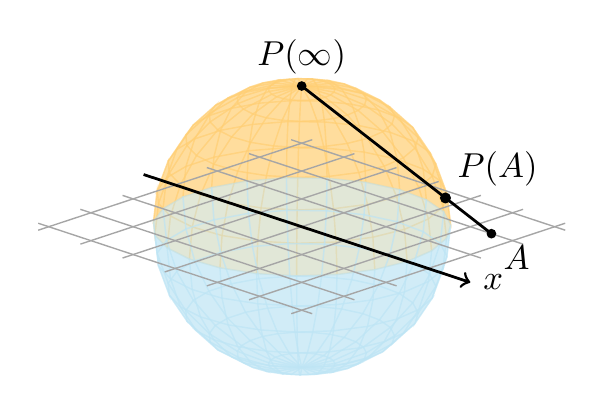
\begin{tikzpicture}[scale=1.25]
        \begin{axis}[
            view={45}{25},
            axis lines=none,
            ticks=none,
            xmin=-1.6, xmax=1.6,
            ymin=-1.6, ymax=1.6,
            zmin=-1.2, zmax=1.2,
            clip=false,
        ]
            \addplot3[surf, shader=flat, color=Orange!55, opacity=0.45, draw=none, samples=24, samples y=8, domain=0:360, y domain=0:90]
                ({sin(y)*cos(x)}, {sin(y)*sin(x)}, {cos(y)});
            \addplot3[surf, shader=flat, color=SkyBlue!55, opacity=0.45, draw=none, samples=24, samples y=8, domain=0:360, y domain=90:180]
                ({sin(y)*cos(x)}, {sin(y)*sin(x)}, {cos(y)});

          
            \addplot3[surf, opacity=0, draw=none, samples=2, domain=-1.3:1.3, y domain=-1.3:1.3]
                ({x}, {y}, {0});
        
            \foreach \t in {-1.2,-0.8,...,1.2} {
                \addplot3[thin, gray!70, domain=-1.3:1.3] ({x}, {\t}, {0});
                \addplot3[thin, gray!70, domain=-1.3:1.3] ({\t}, {x}, {0});
            }

      
            \draw[->, thick] (axis cs:-1.5,0,0) -- (axis cs:1.6,0,0) node[anchor=west] {$x$};

            \coordinate (N) at (axis cs:0,0,1);
            \coordinate (A) at (axis cs:1.0,0.8,0);
            \coordinate (P) at (axis cs:0.758,0.606,0.242);

            \draw[thick] (N) -- (A);

            \fill (N) circle (1.4pt) node[above] {$P(\infty)$};
            \fill (A) circle (1.4pt) node[below right] {$A$};
            \fill (P) circle (1.6pt) node[above right] {$P(A)$};

        \end{axis}
    \end{tikzpicture}
\end{minipage}

\section{平面点集的复数表示}
\subsection{平面曲线}
设曲线$\Gamma$的参数方程为$x = x(t), y = y(t), t\in [\alpha, \beta]$，则用复数$z(t) = x(t) + iy(t)$表示$\Gamma$.
默认曲线$\Gamma$是有向曲线，其正向为参数$t$增大的方向.
以下是几种特殊的平面曲线.
\begin{enumerate}[label=(\arabic*), itemsep=0.5pt]
    \item 简单曲线: 不自交的曲线.
    \item 光滑曲线: $x(t)$和$y(t)$在$[\alpha, \beta]$内处处可导的曲线.
    \item 逐段光滑曲线: 由有限条光滑曲线段相接而成的曲线.
    \item 闭曲线: 起点与终点重合的曲线.
\end{enumerate}

接下来介绍平面直角坐标方程转换为复数方程的方法.
对于参数方程，只需要代入$z(t) = x(t) + iy(t)$化简即可.
\begin{example}
    将$
    \begin{cases}
        x = x_0 + r_0\cos t,\\
        y = y_0 + r_0\sin t,
    \end{cases} t \in [0, 2\pi]$
    转变为复数表示.
\end{example}
\begin{solution}
    \[
        z = x_0 + iy_0 + r_0(\cos t + i\sin t) = z_0 + r_0 e^{it}, \quad t \in [0, 2\pi].
    \qedhere\]
\end{solution}
\begin{example}
    将$\begin{cases}
        x = x_0 + at,\\ 
        y = y_0 + bt,
    \end{cases} t \in [0, 1]$
    转变为复数表示.
\end{example}
\begin{solution}
    \[
        z = x_0 + iy_0 + (a + ib)t = z_0 + ct, \quad t \in [0, 1].
    \]
    其中$z_0 = x_0 + iy_0, c = a + ib$.
\end{solution}  

对于曲线方程$f(x, y) = 0$，只需要代入$x = \frac{z + \overline{z}}{2}, y = \frac{z - \overline{z}}{2i}$，得到$f\left(\frac{z + \overline{z}}{2}, \frac{z - \overline{z}}{2i}\right) = 0$即可.

\begin{example}
    将曲线$x^2 + y^2 = 1$转变为复数表示.
\end{example}
\begin{solution}
    将$$x = \frac{z + \overline{z}}{2}, y = \frac{z - \overline{z}}{2i}$$代入$x^2 + y^2 = 1$，
    得到$$\left(\frac{z + \overline{z}}{2}\right)^2 + \left(\frac{z - \overline{z}}{2i}\right)^2 = 1,$$
    即$z\overline{z} = 1$.
\end{solution}

\begin{example}
    将$\arg{(z - 2i)} = \frac{\pi}{4}$转变为曲线方程.
\end{example}
\begin{solution}
    将$z = x + iy$代入$\arg{(z - 2i)} = \frac{\pi}{4}$，得到
    $$\arg{(x + iy - 2i)} = \frac{\pi}{4},$$
    即$\arctan\left(\frac{y - 2}{x}\right) = \frac{\pi}{4}$，即$y - 2 = x$，即$y = x + 2(x > 0)$.
\end{solution}

\par\vspace{8pt}


\subsection{平面区域}

\noindent\textbf{几种特殊的点:}
\begin{enumerate}[label=(\arabic*), itemsep=1pt]
    \item 点$z_0$的邻域: $U(z_0, \delta) = \{z\vert\left| z - z_0\right| < r \}$.
    \item 点$z_0$的去心邻域: $\mathring{U}(z_0, \delta) = \{z\vert 0 < \left|z - z_0\right| < r \}$.
    \item 内点：点$z_0$是集合$S$的内点$\iff$存在邻域$U(z_0, \delta) \subset S$.
    \item 外点：点$z_0$是集合$S$的外点$\iff$点$z_0$是$S^c$的内点，这里$S^c$是$S$的补集.
    \item 边界点：点$z_0$是集合$S$的边界点$\iff$点$z_0$既不是$S$的内点，也不是$S$的外点.
\end{enumerate}

\noindent\textbf{几种特殊的点集：}
\begin{enumerate}[label=(\arabic*), itemsep=1pt]
   \item 开集: 集合$S$是开集$\iff$集合$S$的每个点都是内点.
   \item 闭集: 集合$S$是闭集$\iff$集合$S^c$为开集.
   \item 边界： 集合$S$的边界$\partial S$是由集合$S$的所有边界点组成的集合.
   \item 闭包： 集合$S$的闭包$\overline{S}$是由$S$和$\partial S$的并集.
   \item 连通集: 集合$S$是连通集$\iff$集合$S$中任意两点都可以用一条完全在$S$内的逐段光滑的曲线连接.
   
   \item 开区域: 集合$S$是开区域$\iff$集合$S$既是开集又是连通集.
   
    \begin{note*}
        开区域简称为区域，区域\textbf{不是}开区域和闭区域的统称.
    \end{note*} 
    \item 闭区域: 集合$S$是闭区域$\iff$集合$S$既是闭集又是连通集.
\end{enumerate}

\begin{note}[区域的连通性]
    如果区域$D$内任意一条简单闭曲线的内部区域完全包含于$D$，则称$D$为\textbf{单连通区域}，否则称$D$为\textbf{多连通区域}.

    直觉上看，多连通区域是包含“洞”的区域，单连通区域是“没有洞”的区域.
\end{note}
\begin{example}[常见的区域]
    \leavevmode\\[6pt]
    \begin{minipage}{0.45\textwidth}
        圆域$B_r(z_0) = \{z\vert |z - z_0| < r\}$.

        \begin{center}
        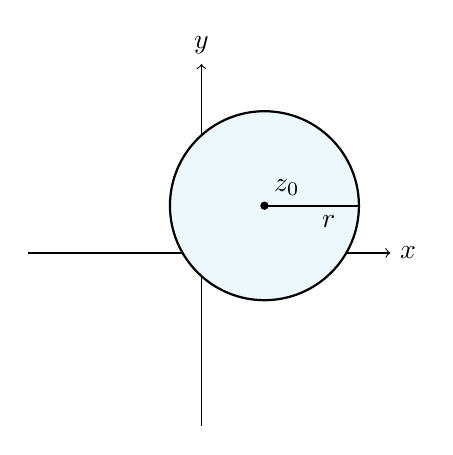
\begin{tikzpicture}[scale=1]
            \draw[->] (-2.2,0) -- (2.4,0) node[right] {$x$};
            \draw[->] (0,-2.2) -- (0,2.4) node[above] {$y$};
            \draw[thick, fill=SkyBlue!15] (0.8,0.6) circle (1.2);
            \fill (0.8,0.6) circle (1.5pt) node[above right] {$z_0$};
            \draw[thick] (0.8,0.6) -- (2.0,0.6) node[midway, below right] {$r$};
        \end{tikzpicture}
        \end{center}
    \end{minipage}
    \begin{minipage}{0.45\textwidth}
        圆环域$A_r(z_0) = \{a < |z - z_0| < b\}$.
        \begin{center}
        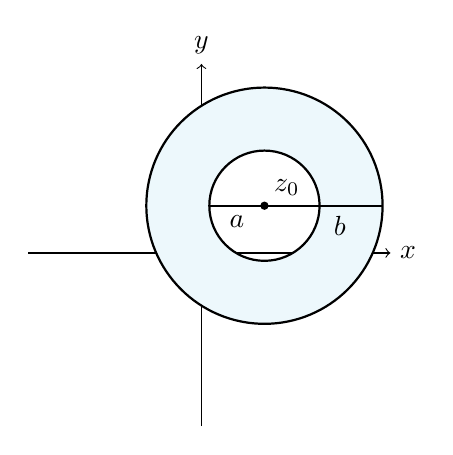
\begin{tikzpicture}[scale=1]
            \draw[->] (-2.2,0) -- (2.4,0) node[right] {$x$};
            \draw[->] (0,-2.2) -- (0,2.4) node[above] {$y$};
            \fill[SkyBlue!15, even odd rule] (0.8,0.6) circle (1.5) (0.8,0.6) circle (0.7);
            \draw[thick] (0.8,0.6) circle (1.5);
            \draw[thick] (0.8,0.6) circle (0.7);
            \fill (0.8,0.6) circle (1.5pt) node[above right] {$z_0$};
            \draw[thick] (0.8,0.6) -- (2.3,0.6) node[midway, below right] {$b$};
            \draw[thick] (0.8,0.6) -- (0.1,0.6) node[midway, below] {$a$};
        \end{tikzpicture}
        \end{center}
    \end{minipage}\par\vspace{8pt}
    \begin{minipage}{0.45\textwidth}
        角形域$D = \{z\vert \alpha < \mathrm{Arg}(z - z_0) < \beta\}$.
        \begin{center}
        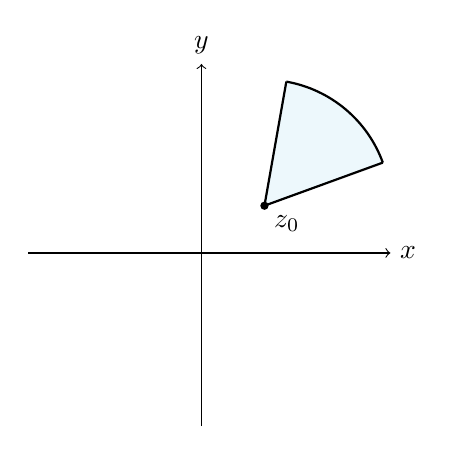
\begin{tikzpicture}[scale=1]
            \draw[->] (-2.2,0) -- (2.4,0) node[right] {$x$};
            \draw[->] (0,-2.2) -- (0,2.4) node[above] {$y$};
            \fill[SkyBlue!15] (0.8,0.6) -- ++(20:1.6) arc (20:80:1.6) -- cycle;
            \draw[thick] (0.8,0.6) -- ++(20:1.6);
            \draw[thick] (0.8,0.6) -- ++(80:1.6);
            \draw[thick] (0.8,0.6) ++(20:1.6) arc (20:80:1.6);
            \fill (0.8,0.6) circle (1.5pt) node[below right] {$z_0$};
        \end{tikzpicture}
        \end{center}
    \end{minipage}
    \begin{minipage}{0.50\textwidth}
        月牙形域$D = \{\left| z - 1 \right| < 1 \}\cap\{\left|z\right| > 1\}$.
        \begin{center}
        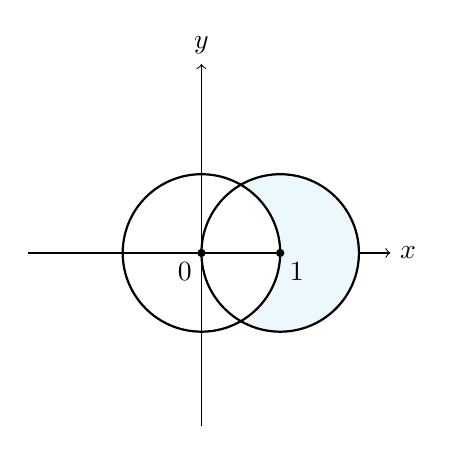
\begin{tikzpicture}[scale=1]
            \draw[->] (-2.2,0) -- (2.4,0) node[right] {$x$};
            \draw[->] (0,-2.2) -- (0,2.4) node[above] {$y$};
            \begin{scope}
                \clip (1,0) circle (1);
                \fill[SkyBlue!15, even odd rule] (-2.2,-2.2) rectangle (2.4,2.4) (0,0) circle (1);
            \end{scope}
            \draw[thick] (1,0) circle (1);
            \draw[thick] (0,0) circle (1);
            \fill (0,0) circle (1.5pt) node[below left] {$0$};
            \fill (1,0) circle (1.5pt) node[below right] {$1$};
        \end{tikzpicture}
        \end{center}
    \end{minipage}
\end{example}\addtocounter{solution}{1}

\section{复变函数}
\subsection{复变函数的定义}
    复数集到复数集的单值对应的映射称为\text{复变函数}，以$w = f(z)$记自变量为$z$的复变函数.

    复变函数可以看作复平面上集合间的映射，但通常不能像一元实函数那样画出图像，因为这需要一个实四维的坐标空间，很难在平面（纸面）上画出示意图.

    复变函数论中，多值对应也是常见的，例如幅角$\mathrm{Arg}(z)$，这种对应关系称为\textbf{多值函数}.
\subsection{复变函数的分量表示}
    给定复变函数$w = f(z)$，记$z = x + iy$，再记$u = \mathrm{Re}(z), v = \mathrm{Im}(z)$，
    则$u$，$v$由(x, y)唯一确定，从而$u$，$v$可看作关于$x, y$的二元实函数.即对应关系$z\to f(z)$等同于
    \[
    \left(
        \begin{array}{l}
            x\\
            y
        \end{array}
    \right)\to
    \left(
        \begin{array}{l}
            u(x, y)\\
            v(x, y)
        \end{array}
    \right).
    \]
\begin{example}
    求直线$y = x$在映射$w = z^{-1}$下的像.
\end{example}
\begin{solution}

    取直线$y = x$的参数方程为$z(t) = (t,t)$，其中$t$为实数，则
    \[
        u = \frac{t}{t^2 + t^2} = \frac{1}{2t}, \qquad
        v = -\frac{t}{t^2 + t^2} = -\frac{1}{2t}.
    \]
    消去参数$t$，得像的方程为
    \[
        u = -v, \qquad (u,v)\neq(0,0),
    \]
    即$w$平面上第二、四象限的角平分线去掉原点.
\end{solution}
\newpage
\chapter{复变函数的微积分}
\section{复变函数及其连续性}
\begin{definition}[复变函数的极限]
设$f(z)$在点$z_0$的某去心邻域内有定义，若$\forall\varepsilon > 0,\exists\delta > 0$，当$0 < |z - z_0| < \delta$时，$|f(z) - w_0| < \varepsilon$，则称$f(z)$在点$z_0$处\textbf{收敛}，并称$w_0$为$f(z)$在点$z_0$处的\textbf{极限}，记为
\[\lim_{z \to z_0} f(z) = w_0.
\]
\end{definition}
\begin{definition}[复变函数的连续性]
  设$f(z)$在点$z_0$有定义，若$\lim_{z \to z_0} f(z) = f(z_0)$，则称$f(z)$在点$z_0$处\textbf{连续}.  
\end{definition}
\par 关于复变函数在无穷远处的极限与连续性，可参考1.2.5节球极投影内容，将$\mathbb{C}$扩展为$\mathbb{C}_\infty$之后再作讨论.
\section{导数与解析函数}
\subsection{复变函数的导数}
\begin{theorem}
设$f(z)$在点$z_0$的某去心邻域内有定义，若极限
\[
    \lim_{z \to z_0} \frac{f(z) - f(z_0)}{z - z_0}
\]
存在，则称$f(z)$在点$z_0$处\textbf{可导}，记极限为$f'(z_0)$，称为$f(z)$在点$z_0$处的\textbf{导数}.
\end{theorem}
与实函数类似，复变函数的导数也满足四则运算、复合函数、反函数等求导法则.
\begin{enumerate}\setlength{\itemsep}{0.5pt}
  \item $(f+g)' = f' + g'$,
  \item $(c)' = 0$,
  \item $(fg)' = f'g + fg'$,
  \item $\left(\dfrac{f}{g}\right)' = \dfrac{f'g - fg'}{g^2}$,
  \item $[f(g(z))]' = f'(g(z))\,g'(z)$,
  \item 若$f$在$z_0$可导，则$f$在$z_0$连续.
\end{enumerate}
\begin{example}
研究函数
$
f(z)=z^3
$的可导性.
\end{example}

\begin{solution}
\par
\textbf{解法一：按导数定义计算}

由导数定义，
\[
f'(z)
=
\lim_{\Delta z\to 0}
\frac{f(z+\Delta z)-f(z)}{\Delta z}.
\]

注意到
\[
f(z+\Delta z)=(z+\Delta z)^3
= z^3+3z^2\Delta z+3z(\Delta z)^2+(\Delta z)^3,
\]
因此
\[
\frac{f(z+\Delta z)-f(z)}{\Delta z}
=
3z^2+3z(\Delta z)+(\Delta z)^2.
\]

令 $\Delta z\to 0$，得
\[
f'(z)=3z^2.
\]

\textbf{解法二：利用 Cauchy--Riemann 方程}

设
\[
f(z)=u(x,y)+iv(x,y),
\quad z=x+iy.
\]
则
\[
u(x,y)=x^3-3xy^2,
\qquad
v(x,y)=3x^2y-y^3.
\]

计算偏导数：
\[
\frac{\partial u}{\partial x}=3x^2-3y^2,
\qquad
\frac{\partial u}{\partial y}=-6xy,
\]
\[
\frac{\partial v}{\partial x}=6xy,
\qquad
\frac{\partial v}{\partial y}=3x^2-3y^2.
\]

可见 Cauchy--Riemann 方程成立，且偏导连续，
因此 $f$ 在 $\mathbb{C}$ 上可导.

由
\[
f'(z)
=
\frac{\partial u}{\partial x}
+
i\frac{\partial v}{\partial x},
\]
得
\[
f'(z)
=
(3x^2-3y^2)+i(6xy)
=
3(x+iy)^2
=
3z^2.
\]
\end{solution}

\subsection{解析函数}
\begin{definition}
$w=f(z)$在$z_0$的某个邻域内处处可导，则称$f(z)$在$z_0$处解析. 若$f(z)$在区域$D$内解析，则称$f(z)$为区域$D$内的\textbf{解析函数}.
\end{definition}
\begin{table}[h!]
    \centering
    \caption{关于解析与可导的概念}
    \begin{tabular}{lcl} % 三列，对齐方式：左-中-左
    \toprule % 顶线（最粗）
    点集类型 & 可导与解析的关系 & 核心原因 \\
    \midrule % 中线（中等粗细）
    区域$D$ & $f(z)$处处可导 $\iff$ $f(z)$解析 & 开集性，邻域完全包含于区域 \\
    单点$z_0$ & $f(z)$解析 $\implies$ 可导；可导 $\nRightarrow$ 解析 & 可导仅单点，邻域内未必可导 \\
    闭区域$\overline{D}$ & 闭区域上解析$\iff$内部$D$解析+边界可导 & 闭区域非开集，边界点无内邻域 \\
    \bottomrule % 底线（最粗，与顶线一致）
  \end{tabular}
\end{table}
以下给出判断复变函数是否是解析函数的一个必要条件.

\begin{theorem}
    设$f(z)=u(x,y)+iv(x,y)$，则$f(z)$在点$z_0=x_0+iy_0$处解析的\textbf{必要条件}是$u,v$在$z_0$处存在且满足\textbf{\text{Cauchy}-\text{Riemaan}(Cauchy-Riemann)方程}:
\[\frac{\partial u}{\partial x} = \frac{\partial v}{\partial y},\quad \frac{\partial u}{\partial y} = -\frac{\partial v}{\partial x}.
\]
\end{theorem}
\begin{proof}[\textbf{证明}]
设$f(z)=u(x,y)+iv(x,y)$在点$z_0=x_0+iy_0$处解析，则$f(z)$在点$z_0$处可导，故
\[f'(z_0) = \lim_{z \to z_0} \frac{f(z) - f(z_0)}{z - z_0}
\]
存在.分别沿$\Delta y=0$和$\Delta x=0$两条路径计算该极限，得
\[\begin{aligned}
    f'(z_0) & = \lim_{\Delta x \to 0} \frac{u(x_0 + \Delta x, y_0) - u(x_0, y_0)}{\Delta x} + i\lim_{\Delta x \to 0} \frac{v(x_0 + \Delta x, y_0) - v(x_0, y_0)}{\Delta x} \\
    & = \frac{\partial u}{\partial x}\bigg|_{(x_0,y_0)} + i\frac{\partial v}{\partial x}\bigg|_{(x_0,y_0)}
\end{aligned}
\]
和
\[\begin{aligned}
    f'(z_0) & = \lim_{\Delta y \to 0} \frac{u(x_0, y_0 + \Delta y) - u(x_0, y_0)}{i\Delta y} + i\lim_{\Delta y \to 0} \frac{v(x_0, y_0 + \Delta y) - v(x_0, y_0)}{i\Delta y} \\
    & = \frac{\partial v}{\partial y}\bigg|_{(x_0,y_0)}
-i\frac{\partial u}{\partial y}\bigg|_{(x_0,y_0)}.
\end{aligned}\]
比较上面两式的实部和虚部，得\text{Cauchy}-\text{Riemann}方程.
\end{proof}
如果加上可微，则这个条件是充要的.
\begin{theorem}
    设$f(z)=u(x,y)+iv(x,y)$，则$f(z)$在点$z_0=x_0+iy_0$处解析的\textbf{充要条件}是$u,v$在点$(x_0,y_0)$处可微，且满足\text{Cauchy}-\text{Riemann}方程.
\end{theorem}


\section{初等函数}
\subsection{指数函数}
\begin{definition}
    对于复数$z = x + iy$，定义指数函数为
\[e^z = e^{x + iy} = e^x(\cos y + i\sin y).\]
\end{definition}
性质：
\begin{enumerate}\setlength{\itemsep}{0.5pt}
  \item $(e^z)' = e^z$，
  \item $e^{z_1 + z_2} = e^{z_1}e^{z_2}$，
  \item 周期性：$e^{z + 2k\pi i} = e^z$($k \in \mathbb{Z}$)，
  \item 值域$\mathbb{C}/\{0\}$.
\end{enumerate}

\subsection{对数函数}
\begin{definition}
  对于复数$z \neq 0$，定义对数函数为
\[\mathrm{Ln} z = \ln|z| + i\, \mathrm{Arg}(z).\]
并称$\ln z = \ln|z| + i\arg(z)$为对数函数的\textbf{主值}.
\end{definition}
性质：
\begin{enumerate}\setlength{\itemsep}{0.5pt}
    \item $(\mathrm{Ln} z)' = \frac{1}{z}$，
    \item $\mathrm{Ln}(z_1z_2) = \mathrm{Ln} z_1 + \mathrm{Ln} z_2 + 2k\pi i$($k \in \mathbb{Z}$)，
    \item $\mathrm{Ln} z = \ln|z| + i(\arg(z) + 2k\pi)$($k \in \mathbb{Z}$)，
    \item 值域$\mathbb{C}$，
\end{enumerate}
\subsection{三角函数}
\begin{definition}
对于复数$z$，定义三角函数
\[
\cos z = \frac{e^{iz} + e^{-iz}}{2}, \quad \sin z = \frac{e^{iz} - e^{-iz}}{2i}
\]
\end{definition}
性质：
\begin{enumerate}\setlength{\itemsep}{0.5pt}
  \item $(\cos z)' = -\sin z$,$(\sin z)' = \cos z$，
  \item 周期性：$\cos(z + 2\pi) = \cos z$,$\sin(z + 2\pi) = \sin z$，
  \item $\cos z$的零点为$z = \frac{\pi}{2} + k\pi$($k \in \mathbb{Z}$)，$\sin z$的零点为$z = k\pi$($k \in \mathbb{Z}$)，
  \item $\sin ^2 z + \cos^2 z = 1$，
  \item 值域$\mathbb{C}$.
\end{enumerate}

\subsection{幂函数}
\begin{definition}
  对于复数$z\neq 0$和$\alpha\in\mathbb{C}$，定义幂函数为
\[z^\alpha = e^{\alpha \mathrm{Ln} z}，\]
且称$e^{\alpha \mathrm{Ln} z}$为幂函数的主值.
\end{definition}
性质：
\begin{enumerate}\setlength{\itemsep}{0.5pt}
    \item 当$\alpha$为整数时，$z^\alpha$为单值的；否则为多值的.
    \item 当$\alpha$为有理数时，$z^\alpha$为有限个值的；否则为无限多值的.
    \item $(z^\alpha)' = \alpha z^{\alpha - 1}$.
    \item 值域$\mathbb{C}$.
\end{enumerate}

\section{解析函数的积分}
\subsection{复积分的定义与计算}
\begin{definition}
  设 $C$ 为复平面上的光滑曲线，$f(z) = u + iv$，记
\[
\int_C f(z)\mathrm{d}z =\lim_{|\Delta z|\rightarrow 0} \sum_{k=1}^n f(z_k)\Delta z_k = \int_C u\mathrm{d}x - v\mathrm{d}y + i\int_C v\mathrm{d}x + u\mathrm{d}y，
\]
称为复变函数$f(z)$沿曲线$C$的\textbf{复积分}.
\end{definition}
以下介绍参数方程法求积分，并给出一道重要例题，在接下来的\textrm{Cauchy}型积分公式中会用到.

设 $z(t) = x(t) + iy(t)$($\alpha \leq t \leq \beta$),则：
\[
\int_C f(z)\mathrm{d}z = \int_\alpha^\beta f(z(t))z'(t)\mathrm{d}t
\]  
\par\vspace{24pt}
\begin{example}
    设 $C$ 为以 $z_0$ 为中心、半径为 $r$ 的正向圆周
\[
|z-z_0|=r,
\]
求积分
\[
\int_C \frac{\mathrm{d}z}{(z-z_0)^n},
\]
\begin{enumerate}[(\arabic*)]
  \item $n=1$；
  \item $n\neq 1$ 为整数.
\end{enumerate}
\end{example}
\begin{solution}
    $C$参数化为$z(t) = z_0 + re^{it}$，其中$t \in [0,2\pi]$.

    \textbf{(1) $n=1$时，} $$\int_C \frac{\mathrm{d}z}{z-z_0} = \int_0^{2\pi} \frac{ire^{it}}{re^{it}} \mathrm{d}t = 2\pi i.$$
    
    \textbf{(2) $n\neq 1$为整数时，} $$\int_C \frac{\mathrm{d}z}{(z-z_0)^n} = \int_0^{2\pi} \frac{ire^{it}}{r^n e^{int}} \mathrm{d}t = ir^{1-n} \int_0^{2\pi} e^{i(1-n)t} \mathrm{d}t = 0.$$
\end{solution}
\subsection{积分与路径无关的条件}
\begin{theorem}[积分与路径无关的条件]\label{jifenlujingwuguan}
    以下条件等价：
    \begin{enumerate}\setlength{\itemsep}{0.5pt}
        \item $\int_C f(z)\mathrm{d}z$ 与路径 $C$ 无关(仅与起点终点有关)
        \item 对 $D$ 内任意闭曲线 $C$,$\int_C f(z)\mathrm{d}z = 0$
        \item 存在 $F(z)$ 使得 $F'(z) = f(z)$($F(z)$ 为 $f(z)$ 的原函数),且 $\int_{z_1}^{z_2} f(z)\mathrm{d}z = F(z_2) - F(z_1)$
    \end{enumerate}
    进一步，若$C$的起点与终点分别为$z_1$与$z_2$，则
    \[
        \int_{z_1}^{z_2} f(z)\mathrm{d}z = F(z_2) - F(z_1).
    \]
\end{theorem}

\section{\text{Cauchy}型积分公式}
\subsection{\text{Cauchy}积分定理}
\begin{theorem}[Cauchy 积分定理]
设 $D$ 为有界区域，$f(z)$ 在 $D$ 内解析，且连续到边界，则
\[
\int_{\partial D} f(z)\,\mathrm{d}z = 0.
\]
\end{theorem}

\begin{proof}[\textbf{证明}]
    由格林公式和C-R方程
    \begin{align*}
        & \int_{\partial D} f(z)\,\mathrm{d}z \\
        = &\int_{\partial D} (u + iv)(\mathrm{d}x + i\mathrm{d}y) \\
        = &\int_{\partial D} u\mathrm{d}x - v\mathrm{d}y + i\int_{\partial D} v\mathrm{d}x + u\mathrm{d}y\\
        \overset{\text{Green}}{=} &\iint_D \left(-\frac{\partial v}{\partial x} - \frac{\partial u}{\partial y}\right) \mathrm{d}x\mathrm{d}y + i\iint_D \left(\frac{\partial u}{\partial x} - \frac{\partial v}{\partial y}\right) \mathrm{d}x\mathrm{d}y \\
       \overset{\text{C-R}}{=} & 0.\qedhere
    \end{align*}
\end{proof}
\subsection{\text{Cauchy}积分公式}
\begin{theorem}
  设 $D$ 为单连通区域,$f(z)$ 在 $D$ 内解析,$z_0 \in D$,$\partial D$ 为简单闭曲线,则
\[
f(z_0) = \frac{1}{2\pi i} \int_{\partial D} \frac{f(z)}{z - z_0}\mathrm{d}z.
\]
\end{theorem}
\begin{proof}[\textbf{证明}]
记
\[
D_1 = D \setminus B_\varepsilon(z_0),
\]
其中 $B_\varepsilon(z_0)=\{z:\,|z-z_0|<\varepsilon\}$.

由于 $f(z)$ 在 $D_1$ 内解析，由 Cauchy 积分定理可得
\[
0
=
\int_{\partial D_1} \frac{f(z)}{z-z_0}\,\mathrm{d}z.
\]
注意到
\[
\partial D_1 = \partial D \cup \{\,|z-z_0|=\varepsilon\,\},
\]
且内边界方向为负向，因此
\[
0
=
\int_{\partial D} \frac{f(z)}{z-z_0}\,\mathrm{d}z
-
\int_{|z-z_0|=\varepsilon} \frac{f(z)}{z-z_0}\,\mathrm{d}z.
\]
即
\[
\int_{\partial D} \frac{f(z)}{z-z_0}\,\mathrm{d}z
=
\int_{|z-z_0|=\varepsilon} \frac{f(z)}{z-z_0}\,\mathrm{d}z.
\]

设
$
z = z_0 + \varepsilon e^{it},
0 \le t \le 2\pi,
$
则
$
\mathrm{d}z = i\varepsilon e^{it}\,\mathrm{d}t.
$
代入得
\[
\int_{|z-z_0|=\varepsilon} \frac{f(z)}{z-z_0}\,\mathrm{d}z
=
\int_0^{2\pi}
\frac{f(z_0+\varepsilon e^{it})}{\varepsilon e^{it}}
\, i\varepsilon e^{it}\,\mathrm{d}t
=
i\int_0^{2\pi} f(z_0+\varepsilon e^{it})\,\mathrm{d}t.
\]
令 $\varepsilon \to 0^+$，并交换积分与极限的次序得
\[
\lim_{\varepsilon\to 0^+}
i\int_0^{2\pi} f(z_0+\varepsilon e^{it})\,\mathrm{d}t
=
2\pi i\, f(z_0).
\]
因此
\[
\boxed{
\int_{\partial D} \frac{f(z)}{z-z_0}\,\mathrm{d}z
=
2\pi i\, f(z_0)
}
\]
\end{proof}

\subsection{\text{Cauchy}高阶导数公式}
\begin{theorem}[\text{Cauchy}高阶导数公式]
条件同前，$n$为整数，有
\[
f^{(n)}(z_0) = \frac{n!}{2\pi i} \int_{\partial D} \frac{f(z)}{(z - z_0)^{n+1}}\mathrm{d}z 
\]
\end{theorem}
\begin{proof}[\textbf{证明}]
将\text{Cauchy}积分公式中的$z_0$看作自变量，两端对$z_0$求$n$阶导数，并交换积分与极限的次序,立即得到
\[f^{(n)}(z_0) 
=\frac{1}{2\pi\mathrm{i}}\frac{\mathrm{d}^n}{\mathrm{d}z_0^n}\int_{\partial D}\frac{f(z)}{z - z_0}\mathrm{d}z
=\frac{1}{2\pi\mathrm{i}}\int_{\partial D}f(z)\frac{\mathrm{d}^n}{\mathrm{d}z_0^n}\left(\frac{1}{z - z_0}\right)\mathrm{d}z 
=\frac{n!}{2\pi i} \int_{\partial D} \frac{f(z)}{(z - z_0)^{n+1}}\mathrm{d}z.\]
\end{proof}
下面介绍一道例题，展示如何在不解析的区域内使用\text{Cauchy}积分定理，并给出通用方法.
\begin{example}
计算 $\int_C \frac{e^z}{(z - 1)(z - 2)}\mathrm{d}z$,其中 $C$ 为：
\begin{enumerate}
  \item $|z| = \frac{1}{2}$,
  \item $|z| = \frac{3}{2}$,
  \item $|z| = 3$.
\end{enumerate}
\end{example}
\begin{solution}
\begin{enumerate}
  \item $|z| = \frac{1}{2}$：被积函数在内部解析,积分 $= 0$
  \item $|z| = \frac{3}{2}$：仅含奇点 $z=1$,积分 $= 2\pi i \cdot \frac{e^z}{z - 2}\bigg|_{z=1} = -2\pi e i$
  \item $|z| = 3$：含奇点 $z=1,z=2$,分解为 $\frac{e^z}{z - 2} - \frac{e^z}{z - 1}$,积分 $= 2\pi i (e^2 - e)$
\end{enumerate}
\end{solution}
根据有理函数的分解定理，有下面介绍的通用的积分公式，看着比较冗长，学习了第三章的留数定理后就会看得比较清楚.
\begin{corollary}
设 $D$ 为有界区域，$f(z)$ 在 $\overline D$ 上解析，
$z_1,\dots,z_k$ 为 $D$ 内互不相同的点，
$\alpha_1,\dots,\alpha_k\in\mathbb{N}$，
且 $z_1,\dots,z_k\notin\partial D$.
则
\[
\int_{\partial D}
\frac{f(z)}
{(z-z_1)^{\alpha_1}\cdots (z-z_k)^{\alpha_k}}
\,\mathrm{d}z
=
2\pi i
\sum_{j=1}^k
\frac{1}{(\alpha_j-1)!}
\frac{\mathrm{d}^{\alpha_j-1}}{\mathrm{d}z^{\alpha_j-1}}
\left(
\frac{f(z)}
{\prod_{m\ne j}(z-z_m)^{\alpha_m}}
\right)
\bigg|_{z=z_j}.\]
\end{corollary}
\subsection{\text{Cauchy}型积分公式的应用}
这一章节介绍几个由\text{Cauchy}型积分公式导出的定理.
\subsubsection{代数学基本定理}
\begin{theorem}
  任意复系数多项式在复平面上至少有一个零点.
\end{theorem}
\begin{proof}[\textbf{证明}]
设
\[
p(z)=a_0 z^n + a_1 z^{n-1} + \cdots + a_n,
\qquad a_0\neq 0,\ a_0,\dots,a_n\in\mathbb{C}.
\]

假设对一切 $z\in\mathbb{C}$，$p(z)\neq 0$.
则 $p(0)\neq 0$，令
\[
f(z)=\frac{1}{p(z)}.
\]
则 $f(z)$ 在 $\mathbb{C}$ 上解析.

由 Cauchy 积分公式，
\[
0\neq f(0)
=
\frac{1}{2\pi i}
\int_{|z|=r}
\frac{f(z)}{z}\,\mathrm{d}z.
\]

设
$
z=re^{it},\quad 0\le t\le 2\pi,
$
则
$
\mathrm{d}z=ire^{it}\,\mathrm{d}t,
$
从而
\[
f(0)
=
\frac{1}{2\pi i}
\int_0^{2\pi}
\frac{f(re^{it})}{re^{it}}
\, ire^{it}\,\mathrm{d}t
=
\frac{1}{2\pi}
\int_0^{2\pi}
f(re^{it})\,\mathrm{d}t.
\]

上式两边令 $r\to +\infty$，并交换积分次序，得
\[
f(0)
=
\frac{1}{2\pi}
\int_0^{2\pi}
\lim_{r\to+\infty}
f(re^{it})\,\mathrm{d}t.
\]

而
\[
\lim_{|z|\to\infty} f(z)
=
\lim_{|z|\to\infty}
\frac{1}{p(z)}
=
0.
\]

因此
\[
f(0)=0,
\]
矛盾.

故假设不成立，结论得证.
\end{proof}
\subsubsection{Liouville 定理}
\begin{definition}
  若函数 $f$ 在 $\mathbb{C}$ 上解析，则称 $f$ 为整函数.
\end{definition}
\begin{theorem}[Liouville 定理]
  若 $f$ 为有界整函数，则 $f$ 为常数函数.
\end{theorem}
\begin{proof}[\textbf{证明}]
设 $f$ 为整函数，且存在常数 $M>0$，使得对一切 $z\in\mathbb{C}$，
$
|f(z)|\le M.
$
则由 Cauchy 导数公式，
\[
f'(z)
=
\frac{1}{2\pi \mathrm{i}}
\int_{|w-z|=r}
\frac{f(w)}{(w-z)^2}\,\mathrm{d}w.
\]

设
$
w=z+re^{it}, \quad 0\le t\le 2\pi,
$则
$
\mathrm{d}w=ire^{it}\,\mathrm{d}t.
$
代入得
\[
f'(z)
=
\frac{1}{2\pi i}
\int_0^{2\pi}
\frac{f(z+re^{it})}{(re^{it})^2}
\, ire^{it}\,\mathrm{d}t
=
\frac{1}{2\pi}
\int_0^{2\pi}
\frac{f(z+re^{it})}{re^{it}}\,\mathrm{d}t
\le
\frac{1}{2\pi}
\int_0^{2\pi}
\frac{|f(z+re^{it})|}{r}\,\mathrm{d}t
\le
\frac{1}{2\pi}
\int_0^{2\pi}
\frac{M}{r}\,\mathrm{d}t
=
\frac{M}{r}.
\]

令 $r\to +\infty$，得
$
f'(z)=0
$，
因此 $f$ 为常数函数，定理得证.
\end{proof}

\subsubsection{Morera定理}
\begin{theorem}
  若函数 $f$ 在区域 $D$ 上连续，且对 $D$ 内任意闭曲线 $\gamma$，
都有
\[
\int_{\gamma} f(z)\,\mathrm{d}z = 0,
\]
则 $f$ 在 $D$ 内解析.
\end{theorem}
\begin{proof}[\textbf{证明}]
由于 $f$ 对任意闭曲线的积分为零，由定理\ref{jifenlujingwuguan}，
可定义
\[
F(z)=\int_{z_0}^{z} f(w)\,\mathrm{d}w，
\]且
\[
F'(z)=f(z).
\]

由于 $F(z)$ 在 $D$ 内解析，故 $f(z)=F'(z)$ 在 $D$ 内解析.
定理得证.
\end{proof}
\section{调和函数}

\begin{definition}
  定义：设 $u(x,y)$ 在区域 $D$ 内二阶连续可微,且满足拉普拉斯方程 $\Delta u = \frac{\partial^2 u}{\partial x^2} + \frac{\partial^2 u}{\partial y^2} = 0$,则称 $u$ 为 $D$ 内的调和函数.

\end{definition}
\begin{note}
  $\Delta$是Laplace算子，对$n$元实函数$h:(x_1,x_2,\cdots,x_n)$，$\Delta h=\Sigma^n_{i=1}\,\frac{\partial^2\,h}{\partial^2\,x_i}$.
\end{note}
\begin{theorem}
若 $f(z) = u + iv$ 在 $D$ 内解析,则 $u$ 和 $v$ 均为 $D$ 内的调和函数,且 $v$ 称为 $u$ 的共轭调和函数.
\end{theorem}
\begin{proof}[\textbf{证明}]
  \( u(x,y),v(x,y) \) 二阶连续可导且

\[
\begin{aligned}
\Delta u &= \frac{\partial^2 u}{\partial x^2} + \frac{\partial^2 u}{\partial y^2} = \frac{\partial}{\partial x}\left(\frac{\partial u}{\partial x}\right) + \frac{\partial}{\partial y}\left(\frac{\partial u}{\partial y}\right) \\
&= \frac{\partial}{\partial x}\left(\frac{\partial v}{\partial y}\right) + \frac{\partial}{\partial y}\left(-\frac{\partial v}{\partial x}\right) = 0
\end{aligned}
\]
类似可证 \(\Delta v = 0\).
\end{proof}
接下来思考一个问题，并由此引出共轭调和函数和解析函数之间的关系.
\begin{problem}如果给定 \( u \)，\( u \) 在 \( D \) 上调和，是否存在 \( v \)，\( v \) 在 \( D \) 上调和，且
\( v \) 为 \( u \) 的共轭调和函数？
\end{problem}
如果 \( v \) 存在，则由 C-R 方程，有
\[
\frac{\partial v}{\partial x} = -\frac{\partial u}{\partial y},\qquad
\frac{\partial v}{\partial y} = \frac{\partial u}{\partial x}.
\]
在 \( D \) 上成立，即 \( -\frac{\partial u}{\partial y}\mathrm{d}x + \frac{\partial u}{\partial x}\mathrm{d}y \) 为 \( v \) 在 \( D \) 上的全微分.

等价于该微分形式在指定区域上积分与路径无关.于是有如下定理.
\begin{theorem}
  当$D$为单连通区域时，$v$必定存在.
\end{theorem}

\begin{example}
已知 $u(x,y) = x^3 - 3xy^2$,求共轭调和函数 $v$ 及解析函数 $f(z)$
\end{example}
\begin{solution}
由 C-R 方程：
\[
\frac{\partial v}{\partial x} = -\frac{\partial u}{\partial y} = 6xy\]
\[\frac{\partial v}{\partial y} = \frac{\partial u}{\partial x} = 3x^2 - 3y^2
\]
积分得 $v = 3x^2y - y^3 + C$($C \in \mathbb{R}$),故 $f(z) = (x^3 - 3xy^2) + i(3x^2y - y^3) + iC = z^3 + iC$.
\end{solution}
\begin{example}
令 \( u(x,y)=\ln(x^2+y^2) \)，证明：不存在 \( \mathbb{R}^2\setminus\{(0,0)\} \) 上的函数
\( v(x,y) \)，使得 \( f(z)=u+iv \) 解析.
\end{example}
\begin{solution}
记
\[
\omega = -\frac{\partial u}{\partial y}\mathrm{d}x + \frac{\partial u}{\partial x}\mathrm{d}y
= -\frac{2y}{x^2+y^2}\mathrm{d}x + \frac{2x}{x^2+y^2}\mathrm{d}y
\]
取 \( C \) 为单位圆周，则
\[
\begin{aligned}
\int_C \omega &= \int_0^{2\pi} -2\sin t \, \mathrm{d}\cos t + 2\cos t \, \mathrm{d}\sin t \\
&= \int_0^{2\pi} 2(\sin^2 t + \cos^2 t) \mathrm{d}t = 4\pi \neq 0
\end{aligned}
\]
故 \( \omega \) 在 \( \mathbb{R}^2\setminus\{(0,0)\} \) 上积分依赖于路径，
因此不存在 \( \mathbb{R}^2\setminus\{(0,0)\} \) 上的 \( v \)，使得 \( \omega = \mathrm{d}v \)，
即 \( u \) 不存在 \( \mathbb{R}^2\setminus\{(0,0)\} \) 上的共轭调和函数.
\end{solution}
\subsection{调和函数的性质}
\subsubsection{解析函数的平均值性质}
\begin{theorem}
设 \( f(z) \) 在区域 \( D \) 内解析，且闭圆盘 \( \{z:|z-z_0|\le r\}\subset D \)，则
\[
f(z_0)=\frac{1}{2\pi}\int_0^{2\pi}f(z_0+re^{it})\mathrm{d}t
\]
\end{theorem}

\begin{proof}[\textbf{证明}]
由 Cauchy 积分公式，
\[
f(z_0)=\frac{1}{2\pi i}\int_{|z-z_0|=r}\frac{f(z)}{z-z_0}\mathrm{d}z
\]
作参数代换 \( z=z_0+re^{it} \)（\( 0\le t\le 2\pi \)），则 \( \mathrm{d}z=ire^{it}\mathrm{d}t \)，代入得
\[
\begin{aligned}
f(z_0)&=\frac{1}{2\pi i}\int_0^{2\pi}\frac{f(z_0+re^{it})}{re^{it}}\cdot ire^{it}\mathrm{d}t\\
&=\frac{1}{2\pi}\int_0^{2\pi}f(z_0+re^{it})\mathrm{d}t
\end{aligned}
\]
\end{proof}
\subsubsection{调和函数的平均值性质}
\begin{theorem}
设 \( u(x,y) \) 在区域 \( D \) 上调和，且闭圆盘 \( \{z:|z-z_0|\le r\}\subset D \)（其中 \( z_0=x_0+iy_0 \)），则
\[
u(x_0,y_0)=\frac{1}{2\pi}\int_0^{2\pi}u(x_0+r\cos t,y_0+r\sin t)\mathrm{d}t
\]
\end{theorem}

\begin{proof}[\textbf{证明}]
只需取在 \( \{z:|z-z_0|\le r\} \) 上的解析函数 \( f(z) \)，使得 \( u(x,y)=\operatorname{Re}f(z) \)，再利用解析函数的平均值性质即可.
\end{proof}
\subsubsection{调和函数的极值原理}
\begin{theorem}
若 \( u(x,y) \) 在 \( D \) 上调和，并连续到边界 \( \partial D \)，则 \( u \) 的最大值、最小值只能在 \( \partial D \) 取到，除非 \( u \) 为常值函数.
\end{theorem}

\begin{proof}[\textbf{证明}]
设 \( z_0=x_0+iy_0 \) 为 \( D \) 内部一点，且 \( u \) 在 \( z_0 \) 处取到最大值.由调和函数的平均值性质，
\[
u(x_0,y_0)=\frac{1}{2\pi}\int_0^{2\pi}u(x_0+r\cos t,y_0+r\sin t)\mathrm{d}t
\]
当 \( \{z:|z-z_0|\le r\}\subset D \) 时，对 \( \{z:|z-z_0|\le r\} \) 上任意一点 \( (x,y) \)，必有 \( u(x,y)=u(x_0,y_0) \).

考虑 \( D \) 上的性质 \( P \)：函数 \( u(x,y) \) 在该点达到最大值.由于 \( D \) 是连通的，性质 \( P \) 在 \( D \) 上处处成立，即 \( u(x,y) \) 为 \( D \) 上的常值函数.
\end{proof}
\subsubsection{最大模原理}
\begin{theorem}
设 \( f(z) \) 在区域 \( D \) 上解析，且连续到边界 \( \partial D \)，则 \( |f(z)| \) 在 \( D \) 上的最大值只能在 \( \partial D \) 达到，除非 \( f \) 为常值函数.
\end{theorem}

\begin{proof}[\textbf{证明}]
由平均值性质，对 \( D \) 内任意点 \( z_0 \)，有
\[
|f(z_0)| \le \frac{1}{2\pi}\int_0^{2\pi}|f(z_0+re^{it})|\mathrm{d}t
\]
类似调和函数的极值原理即可完成证明.
\end{proof}
\subsubsection{调和函数的Liouville定理}
\begin{theorem}
全平面上有上界（或有下界）的调和函数必为常值函数.
\end{theorem}

\begin{proof}[\textbf{证明}]
设 \( u(x,y) \) 在 \( \mathbb{R}^2 \) 上有上界，即 \( u(x,y)\le M \).因 \( \mathbb{R}^2 \) 为单连通区域，存在 \( \mathbb{C} \) 上的解析函数 \( f(z) \)，使得 \( \operatorname{Re}f(z)=u(x,y) \).
考虑 \( g(z)=e^{f(z)} \)，则
\[
|g(z)|=|e^{u+iv}|=e^u\le e^M
\]
由解析函数的 Liouville 定理，\( g(z) \) 为常值函数.设 \( g(z)\equiv C \)，则 \( u=\ln|g(z)|=\ln|C| \)，即 \( u \) 为常值.
\end{proof}
\subsubsection{调和函数无穷阶可导}
\begin{theorem}
若 \( u \) 在区域 \( D \) 上调和，则 \( u \) 在 \( D \) 上无穷次连续可导.
\end{theorem}

\begin{proof}[\textbf{证明}]
由 \( u \) 调和的定义，\( u \) 在局部可表示为某解析函数的实部.由于解析函数本身是无穷次可导的，故其实部 \( u \) 也具有无穷次连续可导性.
\end{proof}
\chapter{解析函数的级数理论和留数定理}
\section{复数项级数与幂级数}
\subsection{复数项级数}
\begin{definition}
  设$\{z_n\}_{n\ge 1}$为一复数列，记$s_n = \sum_{k = 1}^{n}\,z_k$，考虑$\lim_{n\to\infty}s_n$.

  若$\lim_{n\to\infty}s_n$存在，则称级数（记作$\sum_{k = 1}^{\infty}\,z_n$）收敛.
\end{definition}
\begin{example}
几何级数(等比级数)
\[
\sum_{n=1}^{\infty} a_0 q^n = \lim_{N \to \infty} a_0 \frac{1 - q^N}{1 - q}，
\]
\begin{enumerate}
    \item 当 \(|q| < 1\) 时，级数 \(\displaystyle \sum_{n=1}^{\infty} a_0 q^n = \frac{a_0 q}{1 - q}\)
    \item 当 \(|q| \ge 1\) 时，发散
\end{enumerate}
\end{example}
\begin{example}
级数
\[
\sum_{n=1}^{\infty} \frac{1}{n^\alpha} \quad (\alpha > 0)
\]
\begin{enumerate}
    \item \(0 < \alpha \le 1\) 时，发散
    \item \(\alpha > 1\) 时，收敛
\end{enumerate}
\end{example}
\subsection{幂级数}

\begin{definition}
  称形如$\sum_{n=0}^\infty a_n(z - z_0)^n$($a_n \in \mathbb{C}$)的级数为幂级数.
\end{definition}
\begin{theorem}[根植判别法]
  幂级数收敛半径 $R$ 的求法：
\[
\frac{1}{R} = \limsup_{n \to \infty} \sqrt[n]{|a_n|}
\]

\begin{itemize}
  \item 当 $|z - z_0| < R$ 时,级数绝对收敛；
  \item 当 $|z - z_0| > R$ 时,级数发散.
\end{itemize}
\end{theorem}

\begin{theorem}
    幂级数在收敛圆内可以逐项求导、逐项积分,且收敛半径不变.
\end{theorem}
\section{泰勒级数}
\begin{theorem}
若 $f(z)$ 在 $z_0$ 处解析(即存在邻域 $|z - z_0| < r$ 内解析),则在该邻域内：
\[
f(z) = \sum_{n=0}^\infty \frac{f^{(n)}(z_0)}{n!}(z - z_0)^n
\]
称为 $f(z)$ 在 $z_0$ 处的泰勒级数.
\end{theorem}
\begin{proof}[\textbf{证明}]
    由 Cauchy 积分公式，取 $\rho$，使得 $|z-z_0|<\rho<r$，则
\[
f(z) = \frac{1}{2\pi i} \oint_{|w-z_0|=\rho} \frac{f(w)}{w-z} \, \mathrm{d}w
\]

\noindent
注意到
\[
\frac{1}{w-z}
= \frac{1}{(w-z_0) - (z-z_0)}
= \frac{1}{w-z_0} \cdot \frac{1}{1-\dfrac{z-z_0}{w-z_0}}
\quad \left( \frac{|z-z_0|}{|w-z_0|} < 1 \right)
\]
\[
= \frac{1}{w-z_0} \sum_{n=0}^{\infty} \frac{(z-z_0)^n}{(w-z_0)^n}
= \sum_{n=0}^{\infty} \frac{(z-z_0)^n}{(w-z_0)^{n+1}}
\]

\noindent
代入积分可得
\[
f(z)
= \sum_{n=0}^{\infty} \left( \frac{1}{2\pi i} \oint_{|w-z_0|=\rho} \frac{f(w)}{(w-z_0)^{n+1}} \, \mathrm{d}w \right) (z-z_0)^n
= \sum_{n=0}^{\infty} \frac{f^{(n)}(z_0)}{n!} (z-z_0)^n
\]

\end{proof}
常见泰勒展开：
\begin{enumerate}
  \item $e^z = \sum_{n=0}^\infty \frac{z^n}{n!}$($R = +\infty$)
  \item $\sin z = \sum_{n=0}^\infty \frac{(-1)^n z^{2n+1}}{(2n+1)!}$($R = +\infty$)
  \item $\cos z = \sum_{n=0}^\infty \frac{(-1)^n z^{2n}}{(2n)!}$($R = +\infty$)
  \item $\ln(1 - z) = -\sum_{n=1}^\infty \frac{z^n}{n}$($|z| < 1$)
\end{enumerate}
\begin{example}
求 \( f(z)=\dfrac{e^z}{(1-z)^2} \) 在 \( 0 \) 点的 Taylor 级数，并指出收敛半径.
\end{example}

\begin{solution}
已知 \( e^z \) 的 Taylor 展开为
\[
e^z = 1 + z + \frac{z^2}{2!} + \dots + \frac{z^n}{n!} + \dots
\]
\( \dfrac{1}{(1-z)^2} \) 的 Taylor 展开为
\[
\frac{1}{(1-z)^2} = 1 + 2z + 3z^2 + \dots + nz^{n-1} + \dots
\]
将两式相乘可得
\[
\frac{e^z}{(1-z)^2} = 1 + 3z + \frac{11}{2}z^2 + \dots
\]

因 \( f(z) \) 以 \( 0 \) 为中心，在半径最大为 \( 1 \) 的圆盘内解析，故收敛半径为 \( 1 \).
\end{solution}
\begin{example}
求 \( f(z)=\dfrac{1}{1-\sin z} \) 在 \( 0 \) 点的 Taylor 级数，并指出收敛半径.
\end{example}

\begin{solution}
因 \( \sin 0=0 \)，故在 \( 0 \) 的邻域内，满足 \( |\sin z|<1 \).
于是可将 \( \dfrac{1}{1-\sin z} \) 展开为几何级数：
\[
\frac{1}{1-\sin z} = \sum_{n=0}^{\infty} (\sin z)^n
\]
代入 \( \sin z \) 的麦克劳林级数 \( \sin z = z - \frac{z^3}{6} + \dots \)，逐项展开并合并同类项：
\[
\begin{aligned}
\frac{1}{1-\sin z}
&= 1 + \left(z - \frac{z^3}{6} + \dots\right) + \left(z - \frac{z^3}{6} + \dots\right)^2 + \left(z - \frac{z^3}{6} + \dots\right)^3 + \dots \\
&= 1 + z + z^2 + \frac{5}{6}z^3 + \dots
\end{aligned}
\]
该函数离 \( 0 \) 点最近的奇点为 \( z=\dfrac{\pi}{2} \)，故收敛半径为 \( \dfrac{\pi}{2} \).
\end{solution}
\subsubsection{解析函数的零点}

\begin{definition}
若 \( z_0 \) 使得 \( f(z_0)=0 \)，则称 \( z_0 \) 为 \( f(z) \) 的一个 \textbf{零点}.
\end{definition}

考虑 \( f(z) \) 在 \( z_0 \) 处解析，\( z_0 \) 为 \( f(z) \) 的零点，将 \( f(z) \) 在 \( z_0 \) 点写为 Taylor 级数：
\[
f(z) = a_0 + a_1(z-z_0) + a_2(z-z_0)^2 + \dots,\quad |z-z_0|<r
\]

\noindent \textbf{情形 1.}
对一切 \( n \)，\( a_n=0 \)，即 \( f^{(n)}(z_0)=0 \).
故 \( f(z) \) 在 \( |z-z_0|<r \) 内恒为 \( 0 \).
此时由连通性定理，可知 \( f(z)\equiv 0 \).

\noindent \textbf{情形 2.}
\( a_n \) 不全为 \( 0 \)，于是存在 \( m\ge 1 \)，使得 \( a_0=a_1=\dots=a_{m-1}=0 \)，且 \( a_m\neq 0 \).
此时
\[
f(z) = a_m(z-z_0)^m + a_{m+1}(z-z_0)^{m+1} + \dots = (z-z_0)^m \sum_{n=0}^{\infty} a_{m+n}(z-z_0)^n
\]
令 \( g(z) = \sum_{n=0}^{\infty} a_{m+n}(z-z_0)^n \)，则 \( g(z) \) 在 \( |z-z_0|<r \) 内解析，且 \( g(z_0)=a_m\neq 0 \).
即
\[
f(z) = (z-z_0)^m g(z),\quad g(z_0)\neq 0,\; g(z)\text{ 在 }z_0\text{ 解析}
\]
此时 \( z_0 \) 称为 \( f(z) \) 的 $m$\textbf{重零点}，\( m \) 称为零点的 \textbf{重数}.

\( z_0 \) 为 \( f(z) \) 在 \( z_0 \) 的某个邻域上的唯一零点，故是 \textbf{孤立零点}.

\begin{theorem}
非常值的解析函数，零点必 \textbf{孤立}.
\end{theorem}

\begin{corollary}
若 \( f,g \) 在区域 \( D \) 上解析，\( \{z_n\}\subset D \)，\( \lim\limits_{n\to\infty} z_n = z_0\in D \)，且 \( f(z_n)=g(z_n) \)，则 \( f=g \) 在 \( D \) 上成立.
\end{corollary}
\section{\text{Laurent}级数}
\begin{theorem}
  若 $f(z)$ 在圆环域 $r_1 < |z - z_0| < r_2$ 内解析,则在该圆环内：
\[
f(z) = \sum_{n=-\infty}^{+\infty} c_n(z - z_0)^n
\]
其中系数 \[c_n = \frac{1}{2\pi i} \int_C \frac{f(w)}{(w - z_0)^{n+1}}\mathrm{d}w\]
($C$ 为圆环内绕 $z_0$ 的简单闭曲线).
这种形式的级数称为\text{Laurent}级数.
\end{theorem}
\begin{proof}[\textbf{证明}]
  取 $\rho_1, \rho_2$，使得 $r_1<\rho_1<|z-z_0|<\rho_2<r_2$.

由 Cauchy 积分公式，
\[
f(z) = \frac{1}{2\pi i} \oint_{|w-z_0|=\rho_2} \frac{f(w)}{w-z} \, \mathrm{d}w - \frac{1}{2\pi i} \oint_{|w-z_0|=\rho_1} \frac{f(w)}{w-z} \, \mathrm{d}w.
\]

对 $\dfrac{1}{w-z}$ 分情况展开：
\[
\frac{1}{w-z} = \frac{1}{(w-z_0)-(z-z_0)}
=
\begin{cases}
\dfrac{1}{w-z_0} \cdot \dfrac{1}{1-\dfrac{z-z_0}{w-z_0}}
= \displaystyle\sum_{n=0}^{\infty} \frac{(z-z_0)^n}{(w-z_0)^{n+1}}
& \quad (|w-z_0|=\rho_2) \\[12pt]
-\dfrac{1}{z-z_0} \cdot \dfrac{1}{1-\dfrac{w-z_0}{z-z_0}}
= -\displaystyle\sum_{n=0}^{\infty} \frac{(w-z_0)^n}{(z-z_0)^{n+1}}
& \quad (|w-z_0|=\rho_1)
\end{cases}
\]
代入积分并交换积分和求和的次序
\begin{align*}
    f(z) =& \sum_{n=0}^{\infty} \left( \frac{1}{2\pi i} \oint_{|w-z_0|=\rho_2} \frac{f(w)}{(w-z_0)^{n+1}} \, \mathrm{d}w \right) (z-z_0)^n \\
    & + \sum_{n=0}^{\infty} \left( \frac{1}{2\pi i} \oint_{|w-z_0|=\rho_1} f(w)(w-z_0)^n \, \mathrm{d}w \right) \frac{1}{(z-z_0)^{n+1}}\\
    =& \sum_{n=-\infty}^{+\infty} \frac{1}{2\pi i} \int_C \frac{f(w)}{(w-z_0)^{n+1}}\mathrm{d}w(z-z_0)^n
\end{align*}
\end{proof}
\begin{example}
求 \( f(z)=\dfrac{1}{(z-1)(z-2)} \) 在以下各区域上的 Laurent 级数：

\begin{enumerate}
    \item \( 0<|z|<1 \)
    \item \( 1<|z|<2 \)
    \item \( |z|>2 \)
    \item \( 0<|z-1|<1 \)
    
\end{enumerate}

\begin{enumerate}
  \setcounter{enumi}{4}
  \item \( 0<|z-2|<1 \)
    \item \( |z-1|>1 \)
    \item \( |z-2|>1 \)
\end{enumerate}

\end{example}

\begin{solution}
先对 \( f(z) \) 做部分分式分解：
\[
f(z) = \frac{1}{z-2} - \frac{1}{z-1} = \frac{1}{1-z} - \frac{1}{2-z}
\]

\noindent
\textbf{(1) 当 \( 0<|z|<1 \) 时：}
\[
\begin{aligned}
f(z) &= \frac{1}{1-z} - \frac{1}{2} \cdot \frac{1}{1-\dfrac{z}{2}} \\
&= \sum_{n=0}^{\infty} z^n - \sum_{n=0}^{\infty} \frac{z^n}{2^{n+1}} \\
&= \sum_{n=0}^{\infty} \left(1 - \frac{1}{2^{n+1}}\right) z^n
\end{aligned}
\]

\noindent
\textbf{(2) 当 \( 1<|z|<2 \) 时：}
\[
\begin{aligned}
f(z) &= -\frac{1}{z} \cdot \frac{1}{1-\dfrac{1}{z}} - \frac{1}{2} \cdot \frac{1}{1-\dfrac{z}{2}} \\
&= -\sum_{n=0}^{\infty} \frac{1}{z^{n+1}} - \sum_{n=0}^{\infty} \frac{z^n}{2^{n+1}}
\end{aligned}
\]

\noindent
\textbf{(3) 当 \( |z|>2 \) 时：}
\[
\begin{aligned}
f(z) &= -\frac{1}{z} \cdot \frac{1}{1-\dfrac{1}{z}} + \frac{1}{z} \cdot \frac{1}{1-\dfrac{2}{z}} \\
&= \sum_{n=0}^{\infty} \left(2^n - 1\right) \frac{1}{z^{n+1}}
\end{aligned}
\]

\noindent
\textbf{(4) 当 \( 0<|z-1|<1 \) 时：}
\[
\begin{aligned}
f(z) &= \frac{1}{(z-1)-1} \cdot \frac{1}{z-1} \\
&= -\frac{1}{z-1} \sum_{n=0}^{\infty} (z-1)^n \\
&= -\sum_{n=-1}^{\infty} (z-1)^n
\end{aligned}
\]

\noindent
\textbf{(5) 当 \( |z-1|>1 \) 时：}
\[
\begin{aligned}
f(z) &= \frac{1}{z-1} \cdot \frac{1}{1-\dfrac{1}{z-1}} \\
&= \frac{1}{z-1} \sum_{n=0}^{\infty} \frac{1}{(z-1)^n} \\
&= \sum_{n=1}^{\infty} \frac{1}{(z-1)^n}
\end{aligned}
\]

\noindent
\textbf{(6) 当 \( 0<|z-2|<1 \) 时：}
\[
\begin{aligned}
f(z) &= \frac{1}{z-2} - \frac{1}{(z-2)+1} \\
&= \frac{1}{z-2} - \sum_{n=0}^{\infty} (-1)^n (z-2)^n \\
&= \sum_{n=-1}^{\infty} (-1)^{n+1} (z-2)^n
\end{aligned}
\]

\noindent
\textbf{(7) 当 \( |z-2|>1 \) 时：}
\[
\begin{aligned}
f(z) &= \frac{1}{z-2} - \frac{1}{z-2} \cdot \frac{1}{1+\dfrac{1}{z-2}} \\
&= \frac{1}{z-2} \sum_{n=0}^{\infty} \frac{(-1)^n}{(z-2)^n} \\
&= \sum_{n=1}^{\infty} \frac{(-1)^{n-1}}{(z-2)^n}
\end{aligned}
\]
\end{solution}

\begin{example}
求 \( f(z)=\dfrac{e^z}{(z-1)^2} \) 在 \( |z-1|>0 \) 上的 Laurent 级数.
\end{example}

\begin{solution}
首先，将 \( e^z \) 在 \( z=1 \) 处展开为 Taylor 级数：
\[
e^z = \sum_{n=0}^{\infty} \frac{\left.(e^z)^{(n)}\right|_{z=1}}{n!} (z-1)^n
= \sum_{n=0}^{\infty} \frac{e}{n!} (z-1)^n
\]
将其代入 \( f(z) \) 的表达式并整理：
\[
f(z) = \frac{e^z}{(z-1)^2}
= \sum_{n=0}^{\infty} \frac{e}{n!} (z-1)^{n-2}
\]
\end{solution}
\section{孤立奇点}
\subsection{孤立奇点的类型}
\begin{definition}
  若 $f(z)$ 在 $D$ 内解析,但在 $z_0\in D$ 处不解析,则称 $z_0$ 为 $f(z)$ 的奇点.
\end{definition}
\begin{note}
  函数在奇点处可以有定义
\end{note}
\begin{definition}
  若 $f(z)$ 在 $z_0$ 的某去心邻域 $0 < |z - z_0| < \delta$ 内解析,但在 $z_0$ 处不解析,则称 $z_0$ 为 $f(z)$ 的孤立奇点.
\end{definition}
孤立奇点的分类(按\text{Laurent}级数)
对于 $f(z)$ 的孤立奇点 $z_0$,在 $0 < |z - z_0| < \delta$ 内的\text{Laurent}级数为：
\[
f(z) = \sum_{n=-\infty}^{+\infty} c_n(z - z_0)^n
\]

那么可将$f(z)$的极点分为如下三种.
\begin{definition}
  \begin{enumerate}
  \item 可去奇点：\text{Laurent}级数无负幂项(对所有 $n < 0,c_n = 0$ )
  \item 极点($m$ 级)：\text{Laurent}级数负幂项最高次为 $-m$($c_{-m} \neq 0$,$c_n = 0$ 对 $n < -m$), $m$称为该极点的级
  \item 本性奇点：\text{Laurent}级数有无穷多负幂项
\end{enumerate}
\end{definition}
对于三类极点有各自的判定定理如下.
\begin{theorem}
设 $z_0$ 为函数 $f(z)$ 的孤立点，则：
\begin{enumerate}
  \item $z_0$ 为可去奇点，当且仅当
  \[
    \lim_{z \to z_0} f(z) \ \text{存在}.
  \]

  \item $z_0$ 为极点，当且仅当
  \[
    \lim_{z \to z_0} f(z) = \infty.
  \]

  \item $z_0$ 为本性奇点，当且仅当
  \[
    \lim_{z \to z_0} f(z) \ \text{不存在且不为 } \infty.
  \]
\end{enumerate}
\end{theorem}
\begin{proof}[\textbf{证明}]
设 $z_0$ 为函数 $f(z)$ 的孤立奇点，$f(z)$ 在 $0<|z-z_0|<R$ 内解析，
其\text{Laurent}展开为
\[
f(z)=\sum_{n=-\infty}^{+\infty} C_n (z-z_0)^n .
\]

\textbf{(1) 可去奇点的情形}

若 $z_0$ 为可去奇点，则 $f(z)$ 在 $z_0$ 的邻域内有界，
于是
\[
f(z)=\sum_{n=0}^{+\infty} C_n (z-z_0)^n .
\]
因此
\[
\lim_{z\to z_0} f(z)=C_0 .
\]

反之，若
\[
\lim_{z\to z_0} f(z)=C \quad (\text{有限}),
\]
则由\text{Laurent}系数公式
\[
C_{-n}=\frac{1}{2\pi i}\int_{|z-z_0|=\delta} f(z)(z-z_0)^{n-1}\,\mathrm{d}z,
\quad n\ge1,
\]
并利用 $|f(z)|\le M$，可得
\[
|C_{-n}|
\le \frac{1}{2\pi} \int_{|z-z_0|=\delta} |f(z)|\cdot |z-z_0|^{n-1}\,|\mathrm{d}z|
\le \frac{1}{2\pi} \int_{|z-z_0|=\delta} M\cdot \delta^{n-1}\,|\mathrm{d}z|
= \frac{1}{2\pi}\, M\,\delta^{\,n-1}\cdot 2\pi\delta
= M\delta^{\,n}.
\]
故 $C_{-n}=0$，从而 $z_0$ 为可去奇点.

\medskip
\textbf{(2) 极点的情形}

设 $z_0$ 为 $f(z)$ 的$m$阶极点，则在 $z_0$ 的去心邻域内，
存在正整数 $m$，使得
\[
f(z)=\sum_{n=-m}^{+\infty} C_n (z-z_0)^n,
\qquad C_{-m}\neq 0.
\]

于是
\[
f(z)
=\frac{1}{(z-z_0)^m}
\left[
\sum_{n=-m}^{+\infty} C_n (z-z_0)^{n+m}
\right].
\]
记
\[
g(z)=\sum_{n=-m}^{+\infty} C_n (z-z_0)^{n+m}.
\]
则 $g(z)$ 在 $z_0$ 处解析，且
\[
g(z_0)=C_{-m}\neq 0.
\]
因此
\[
\lim_{z\to z_0} f(z)
= \lim_{z\to z_0} \frac{g(z)}{(z-z_0)^m}
= \infty.
\]

又设
\[
F(z)=\frac{1}{f(z)}.
\]
则
\[
\lim_{z\to z_0} F(z)=0.
\]
由 (1) 知，$z_0$ 为 $F(z)$ 的可去奇点，
从而 $F(z)$ 在 $z_0$ 的某邻域内解析，且
\[
F(z)=\sum_{n=m}^{+\infty} C_n (z-z_0)^n,
\qquad m\ge1,\ C_m\neq 0.
\]

于是
\[
F(z)
=(z-z_0)^m
\left[
\sum_{n=m}^{+\infty} C_n (z-z_0)^{n-m}
\right].
\]
记
\[
G(z)=\sum_{n=m}^{+\infty} C_n (z-z_0)^{n-m},
\]
则 $G(z)$ 在 $z_0$ 处解析，且
\[
G(z_0)=C_m\neq 0.
\]

于是
\[
f(z)=\frac{1}{F(z)}
=\frac{1}{(z-z_0)^m}\cdot \frac{1}{G(z)}.
\]
令
\[
g(z)=\frac{1}{G(z)},
\]
则 $g(z)$ 在 $z_0$ 处解析，且
\[
g(z_0)=\frac{1}{G(z_0)}=\frac{1}{C_m}\neq 0.
\]
因此在 $z_0$ 的去心邻域内，
\[
g(z)=\sum_{n=0}^{+\infty} a_n (z-z_0)^n,
\qquad a_0\neq 0.
\]


\medskip
\textbf{(3) 本性奇点的情形}

若 $z_0$ 为本性奇点，则\text{Laurent}展开中
负次项无限多，
\[
f(z)=\sum_{n=-\infty}^{+\infty} C_n (z-z_0)^n,
\]
从而极限
\[
\lim_{z\to z_0} f(z)
\]
不存在，且不为无穷大.
\end{proof}
\begin{corollary}
\begin{enumerate}
  \item 若 $z_0$ 为可去奇点，则重新定义
  \[
  f(z_0)=\lim_{z\to z_0} f(z),
  \]
  可使 $f$ 在 $z_0$ 解析.

  \item 若 $z_0$ 为 $m$ 阶极点，则
  \[
  f(z)=\frac{g(z)}{(z-z_0)^m},
  \]
  其中 $g(z)$ 在 $z_0$ 解析且 $g(z_0)\neq 0$.
\end{enumerate}
\end{corollary}


\begin{example}
分析下列函数的奇点（位置与类型）：
\begin{enumerate}
    \item \( f(z)=\dfrac{1}{(z-1)(z-2)} \)
    \newline
    奇点为 \( z=1, z=2 \)，均为孤立奇点，且为1级极点.

    \item \( f(z)=\dfrac{\sin z}{z} \)
    \newline
    奇点为 \( z=0 \)，为可去奇点（因 \( \dfrac{\sin z}{z}=1-\dfrac{z^2}{6}+\dots \) 在 \( z=0 \) 邻域解析）.

    \item \( f(z)=\sin\dfrac{1}{z} \)
    \newline
    奇点为 \( z=0 \)，为孤立奇点，且为本性奇点（因 \( \sin\dfrac{1}{z}=\displaystyle\sum_{n=0}^{\infty}\frac{(-1)^n}{(2n+1)!}\frac{1}{z^{2n+1}} \) 含无穷多负幂次项）.

    \item \( f(z)=\dfrac{1}{\sin\dfrac{1}{z}} \)
    \newline
    奇点为 \( z=0 \) 及 \( z=\dfrac{1}{k\pi} \ (k=\pm1,\pm2,\dots) \)；
    其中 \( z=0 \) 非孤立奇点，\( z=\dfrac{1}{k\pi} \) 为1级极点.

    \item \( f(z)=\dfrac{1}{\sin z} \)
    \newline
    奇点为 \( z=k\pi \ (k\in\mathbb{Z}) \)，均为孤立奇点，且为1级极点；
    \( z=\infty \) 为非孤立奇点.

    \item \( f(z)=\ln z \)
    \newline
    奇点为一切负实数和 \( z=0 \)，均为非孤立奇点；
    \( z=\infty \) 为非孤立奇点.
\end{enumerate}
\end{example}
\begin{theorem}
设
\[
f(z)=\frac{g(z)}{h(z)},
\]
其中 $g(z),h(z)$ 在 $z_0$ 的邻域内解析，且
\[
h(z_0)=0.
\]
则有以下结论：
\begin{enumerate}
  \item 若 $g(z_0)\neq 0$，则 $z_0$ 为 $f(z)$ 的极点.
  进一步，若 $h(z)$ 在 $z_0$ 处为 $m$ 重零点，
  则 $z_0$ 为 $f(z)$ 的 $m$ 阶极点.

  \item 若 $g(z_0)=0$，设 $g(z),h(z)$ 分别在 $z_0$ 处为
  $m_1,m_2$ 重零点，则：
  \begin{enumerate}
    \item 若 $m_1\ge m_2$，则 $z_0$ 为 $f(z)$ 的可去奇点；
    \item 若 $m_2>m_1$，则 $z_0$ 为 $f(z)$ 的 $(m_2-m_1)$ 阶极点.
  \end{enumerate}
\end{enumerate}
\end{theorem}
\begin{example}
研究极限
\[
\lim_{z\to 0} z\sin\frac{1}{z}.
\]
在原点处及无穷远点处的情形.
\end{example}

\begin{solution}
因
\[
\sin\frac{1}{z}
= \frac{1}{z}-\frac{1}{6}\frac{1}{z^3}+\cdots,
\]
故
\[
z\sin\frac{1}{z}
= z\left(\frac{1}{z}-\frac{1}{6}\frac{1}{z^3}+\cdots\right)
= 1-\frac{1}{6}\frac{1}{z^2}+\cdots.
\]

因此，$0$ 为 $z\sin\frac{1}{z}$ 的本性奇点，
从而
\[
\lim_{z\to 0} z\sin\frac{1}{z}
\]
不存在，也不为 $\infty$.

$\infty$ 作为孤立奇点的情形与此类似.
\end{solution}

\subsection{无穷远点作为孤立奇点的类型}
$\infty$ 总看作复变函数的一个奇点.
\begin{definition}
若函数 $f(z)$ 在 $|z|>R$ 上解析，则称 $\infty$ 为 $f(z)$ 的孤立奇点.
\end{definition}
\begin{remark}
若 $f(z)$ 在扩充复平面上只有有限个奇点，则一切奇点均孤立；若有无限个奇点，则必有非孤立奇点.
\end{remark}
\begin{definition}
设函数 $f(z)$ 在 $|z|>R$ 上解析，且在无穷远处有\text{Laurent}展开
\[
f(z)=\sum_{n=-\infty}^{+\infty} c_n z^n. \tag{$*$}
\]

设 $f(z)$ 在 $|z|>R$ 上解析，其在无穷远处的\text{Laurent}展开如 $(*)$ 所示，则：
\begin{enumerate}
  \item 若 $(*)$ 式右端无正幂项，
  则 $\infty$ 为 $f(z)$ 的可去奇点；

  \item 若仅有有限个正幂项，
  则 $\infty$ 为 $f(z)$ 的极点；

  \item 若正幂项无限多，
  则 $\infty$ 为 $f(z)$ 的本性奇点.
\end{enumerate}
\end{definition}
当 $\infty$ 为 $f(z)$ 的孤立奇点时，令
\[
w=\frac{1}{z}, \qquad g(w)=f\!\left(\frac{1}{w}\right),
\]
则 $w=0$ 为 $g(w)$ 的孤立奇点，
且其类型与 $\infty$ 作为 $f(z)$ 的奇点类型完全一致.


\section{留数定理}
\subsection{留数定理和几种计算留数的方式}
\begin{definition}
设 $f(z)$ 在去心圆盘
\[
0<|z-z_0|<\varepsilon
\]
内解析，则称
\[
\operatorname{Res}(f,z_0)
=\frac{1}{2\pi i}\int_{|z-z_0|=\varepsilon} f(z)\,\mathrm{d}z
\]
为 $f(z)$ 在 $z_0$ 处的留数.
\end{definition}
\begin{theorem}[留数定理]
设 $C$ 为一简单闭曲线，$f(z)$ 在 $C$ 及其内部除有限个孤立奇点
\[
z_1,z_2,\dots,z_m
\]
外解析，则
\[
\int_C f(z)\,\mathrm{d}z
=2\pi i \sum_{k=1}^{m} \operatorname{Res}(f,z_k).
\]
\end{theorem}

\begin{theorem}
若函数 $f(z)$ 在 $z_0$ 的去心邻域内有\text{Laurent}展开
\[
f(z)=\sum_{n=-\infty}^{+\infty} c_n (z-z_0)^n,
\]
则
\[
\operatorname{Res}(f,z_0)=c_{-1}.
\]
\end{theorem}
\begin{proposition}
若
\[
f(z)=\frac{g(z)}{(z-z_0)^{n+1}},
\]
其中 $n$ 为非负整数，$g(z)$ 在 $z_0$ 处解析，
则
\[
\operatorname{Res}\!\left(\frac{g(z)}{(z-z_0)^{n+1}},z_0\right)
=\frac{g^{(n)}(z_0)}{n!}.
\]
\end{proposition}
\begin{proposition}\label{mingti2}
若
\[
f(z)=\frac{g(z)}{h(z)},
\]
其中 $g(z),h(z)$ 在 $z_0$ 处解析，
\[
h(z_0)=0,\qquad h'(z_0)\neq 0,
\]
则
\[
\operatorname{Res}(f,z_0)=\frac{g(z_0)}{h'(z_0)}.
\]
\end{proposition}
\begin{proof}[\textbf{证明}]
由条件 $h(z_0)=0,\ h'(z_0)\neq 0$，
可写
\[
h(z)=(z-z_0)\,\tilde h(z),
\]
其中 $\tilde h(z)$ 在 $z_0$ 处解析，且
\[
\tilde h(z_0)\neq 0.
\]
于是
\[
f(z)=\frac{g(z)}{(z-z_0)\tilde h(z)}
=\frac{1}{z-z_0}\cdot\frac{g(z)}{\tilde h(z)}.
\]
由于 $\dfrac{g(z)}{\tilde h(z)}$ 在 $z_0$ 处解析，
故
\[
\operatorname{Res}(f,z_0)
=\left.\frac{g(z)}{\tilde h(z)}\right|_{z=z_0}
=\frac{g(z_0)}{\tilde h(z_0)}.
\]

另一方面，由
\[
h'(z)=\tilde h(z)+(z-z_0)\tilde h'(z),
\]
取 $z=z_0$ 得
\[
h'(z_0)=\tilde h(z_0).
\]
因此
\[
\operatorname{Res}(f,z_0)=\frac{g(z_0)}{h'(z_0)}.
\]
\end{proof}
\begin{example}
求
\[
\operatorname{Res}\!\left(\frac{1}{\sin z},\,k\pi\right).
\]
\end{example}

\begin{solution}
由命题\ref{mingti2}知，
\[
\operatorname{Res}\!\left(\frac{1}{\sin z},\,k\pi\right)
=\left.\frac{1}{\cos z}\right|_{z=k\pi}
=(-1)^k.
\]
\end{solution}
\begin{example}
计算积分
\[
I=\oint_{|z|=2}\frac{\mathrm{d}z}{z^5-1}.
\]
\end{example}

\begin{solution}
由留数定理，
\[
I
=2\pi i \sum_{k=0}^{4}
\operatorname{Res}\!\left(\frac{1}{z^5-1},\,e^{\frac{2k\pi i}{5}}\right).
\]

由于
\[
(z^5-1)'=5z^4,
\]
故
\[
\operatorname{Res}\!\left(\frac{1}{z^5-1},\,z_k\right)
=\left.\frac{1}{5z^4}\right|_{z=z_k},
\quad z_k=e^{\frac{2k\pi i}{5}}.
\]

于是
\[
I
=2\pi i \sum_{k=0}^{4}
\frac{1}{5}e^{-\frac{8k\pi i}{5}}
=\frac{2\pi i}{5}\sum_{k=0}^{4} e^{\frac{2k\pi i}{5}}
=0.
\]
\end{solution}


\subsection{无穷远点的留数}
\begin{definition}
设函数 $f(z)$ 在 $|z|>R$ 上解析，则定义
\[
\operatorname{Res}(f,\infty)
=-\frac{1}{2\pi i}\int_{|z|=\rho} f(z)\,\mathrm{d}z,
\qquad \rho>R.
\]
\end{definition}
\begin{theorem}
设 $f(z)$ 在 $|z|>R$ 上有\text{Laurent}展开
\[
f(z)=\sum_{n=-\infty}^{+\infty} c_n z^n,
\]
则
\[
\operatorname{Res}(f,\infty)=-c_{-1}.
\]
\end{theorem}
\begin{remark}
设
\[
g(w)=f\!\left(\frac{1}{w}\right),
\]
则 $g(w)$ 在 $w=0$ 的去心邻域内有\text{Laurent}展开
\[
g(w)=\sum_{n=-\infty}^{+\infty} \frac{C_n}{w^n}.
\]
因此
\[
\operatorname{Res}(g,0)=C_1 \neq \operatorname{Res}(f,\infty).
\]

并且有恒等式
\[
\operatorname{Res}(f,\infty)
=\operatorname{Res}\!\left(-\frac{1}{w^2}f\!\left(\frac{1}{w}\right),\,0\right).
\]
\end{remark}
\begin{corollary}
若函数 $f(z)$ 在扩充复平面 $\overline{\mathbb C}$ 上
仅有有限个孤立奇点
\[
z_1,z_2,\dots,z_m,\ \infty,
\]
则
\[
\sum_{k=1}^{m} \operatorname{Res}(f,z_k)
+\operatorname{Res}(f,\infty)
=0.
\]
\end{corollary}

\section{留数定理在计算实积分中的应用}
\subsection{$
\int_{-\infty}^{+\infty}\frac{P(x)}{Q(x)}\,\mathrm{d}x
$ 类型}
\begin{proposition}
\[
\int_{-\infty}^{+\infty}\frac{P(x)}{Q(x)}\,\mathrm{d}x
=2\pi i\sum_{j=1}^{m}
\operatorname{Res}\!\left(\frac{P(z)}{Q(z)},z_j\right),
\]
其中求和取遍上半平面内的全部极点，且
$
\deg P(x)\le \deg Q(x)-2.
$
\end{proposition}
考虑复积分
\[
\int_{C_R}\frac{P(z)}{Q(z)}\,\mathrm{d}z,
\]
其中 $C_R$ 为由区间 $[-R,R]$ 与上半圆
$
\Gamma_R=\{z:|z|=R,\text{Im}(z)\ge0\}
$
组成的正向闭合曲线.

当 $R$ 充分大时，假设 $Q(z)$ 在上半平面内仅有有限个零点
\[
z_1,z_2,\dots,z_m,
\]
且均包含于 $C_R$ 内.

由留数定理，
\[
\int_{C_R}\frac{P(z)}{Q(z)}\,\mathrm{d}z
=2\pi i\sum_{j=1}^{m}
\operatorname{Res}\!\left(\frac{P(z)}{Q(z)},z_j\right).
\]

另一方面，
\[
\int_{C_R}\frac{P(z)}{Q(z)}\,\mathrm{d}z
=\int_{-R}^{R}\frac{P(x)}{Q(x)}\,\mathrm{d}x
+\int_{\Gamma_R}\frac{P(z)}{Q(z)}\,\mathrm{d}z.
\]

设
\[
P(z)=a_m z^m+\cdots+a_1 z+a_0,\qquad
Q(z)=b_n z^n+\cdots+b_1 z+b_0,
\]
其中 $m\le n-2$.
当 $|z|=R$ 足够大时，存在常数 $M>0$，使得
\[
\left|\frac{P(z)}{Q(z)}\right|
\le \frac{M}{R^2}.
\]

于是
\[
\left|\int_{\Gamma_R}\frac{P(z)}{Q(z)}\,\mathrm{d}z\right|
\le \int_{\Gamma_R}\left|\frac{P(z)}{Q(z)}\right||\mathrm{d}z|
\le \frac{M}{R^2}\cdot \pi R
=\frac{M}{R}
\xrightarrow[R\to\infty]{}0.
\]

因此令 $R\to\infty$，得
\[
\int_{-\infty}^{+\infty}\frac{P(x)}{Q(x)}\,\mathrm{d}x
=2\pi i\sum_{j=1}^{m}
\operatorname{Res}\!\left(\frac{P(z)}{Q(z)},z_j\right),
\]
其中求和取遍上半平面内的全部极点.
\begin{example}
  计算
\[
\int_{-\infty}^{+\infty} \frac{1}{x^4+1}\,\mathrm{d}x .
\]
\end{example}
\begin{solution}
  考虑函数
\[
f(z)=\frac{1}{z^4+1}.
\]
取上半平面的半圆闭合路径 $C$，则由留数定理，
\[
\int_{-\infty}^{+\infty} \frac{1}{x^4+1}\,\mathrm{d}x
= 2\pi i \sum \operatorname{Res}\left( \frac{1}{z^4+1}, z_k \right),
\]
其中 $z_k$ 为 $f(z)$ 在上半平面内的孤立奇点.

方程
\[
z^4+1=0
\]
的根为
\[
z = e^{i\pi/4},\; e^{i3\pi/4},\; e^{i5\pi/4},\; e^{i7\pi/4}.
\]
其中位于上半平面的为
\[
z_1 = e^{i\pi/4}, \qquad z_2 = e^{i3\pi/4}.
\]

由于这些都是一阶极点，
\[
\operatorname{Res}\left( \frac{1}{z^4+1}, z_k \right)
= \left. \frac{1}{(z^4+1)'} \right|_{z=z_k}
= \left. \frac{1}{4z^3} \right|_{z=z_k}.
\]

因此
\[
\int_{-\infty}^{+\infty} \frac{1}{x^4+1}\,\mathrm{d}x
= 2\pi i \left[
\left. \frac{1}{4z^3} \right|_{z=e^{i\pi/4}}
+
\left. \frac{1}{4z^3} \right|_{z=e^{i3\pi/4}}
\right].
\]

计算得
\[
= \frac{\pi i}{2}
\left(
- e^{-3i\pi/4} - e^{-9i\pi/4}
\right)
= -\frac{\pi i}{2}\,\sqrt{2}\, i
= \frac{\pi\sqrt{2}}{2}.
\]

\[
\boxed{
\int_{-\infty}^{+\infty} \frac{1}{x^4+1}\,\mathrm{d}x
= \frac{\pi\sqrt{2}}{2}
}
\]
\end{solution}

\subsection{$
\int_{0}^{+\infty}\frac{P(x)}{Q(x)}\,\mathrm{d}x
$ 类型}
\begin{proposition}
\[
\int_0^{+\infty} \frac{P(x)}{Q(x)}\,\mathrm{d}x
=
- \sum_{k=1}^n
\operatorname{Res}\!\left(
\frac{P(z)}{Q(z)} \log z , z_k
\right).
\]
其中$Q(z)$ 的零点不在正实轴上，右侧求和取遍$Q(z)$的所有零点.
\end{proposition}
考虑复积分
\[
\int_{C_R} \frac{P(z)}{Q(z)} \log z \, \mathrm{d}z,
\]
其中 $C_R$ 为绕过正实轴的钥匙孔型闭合路径.
由留数定理，
\[
\int_{C_R} \frac{P(z)}{Q(z)} \log z \, \mathrm{d}z
= 2\pi i \sum_{k=1}^n
\operatorname{Res}\!\left( \frac{P(z)}{Q(z)} \log z , z_k \right).
\]

将路径分解为各段积分，有
\[
\int_{C_R} \frac{P(z)}{Q(z)} \log z \, \mathrm{d}z
=
\int_0^R \frac{P(x+i\varepsilon)}{Q(x+i\varepsilon)} \log(x+i\varepsilon)\,\mathrm{d}x
+ \int_{\Gamma_R} \frac{P(z)}{Q(z)} \log z\,\mathrm{d}z
\]
\[
\quad
- \int_0^R \frac{P(x-i\varepsilon)}{Q(x-i\varepsilon)} \log(x-i\varepsilon)\,\mathrm{d}x
+ \int_{-\varepsilon}^{\varepsilon}
\frac{P(x_0+i y)}{Q(x_0+i y)} \log(x_0+i y)\,\mathrm{d}z .
\]

取
\[
\log z = \ln|z| + i\arg z, \qquad \arg z \in (0,2\pi),
\]
并令 $R\to +\infty$，$\varepsilon\to 0^+$.

于是有
\[
\int_0^R \frac{P(x+i\varepsilon)}{Q(x+i\varepsilon)} \log(x+i\varepsilon)\,\mathrm{d}x
\longrightarrow
\int_0^{+\infty} \frac{P(x)}{Q(x)} \log x\,\mathrm{d}x,
\]
\[
\int_0^R \frac{P(x-i\varepsilon)}{Q(x-i\varepsilon)} \log(x-i\varepsilon)\,\mathrm{d}x
\longrightarrow
\int_0^{+\infty} \frac{P(x)}{Q(x)} (\log x + 2\pi i)\,\mathrm{d}x.
\]

并且有估计
\[
\left| \frac{P(z)}{Q(z)} \log z \right|
\le \frac{M}{R^2} |\log R + i\theta|
\longrightarrow 0
\qquad (R\to +\infty),
\]
以及
\[
\int_{-\varepsilon}^{\varepsilon}
\frac{P(x_0+i y)}{Q(x_0+i y)} \log(x_0+i y)\,\mathrm{d}z
\longrightarrow 0
\qquad (\varepsilon\to 0^+).
\]

因此得到
\[
\int_0^{+\infty} \frac{P(x)}{Q(x)}\,\mathrm{d}x
=
- \sum_{k=1}^n
\operatorname{Res}\!\left(
\frac{P(z)}{Q(z)} \log z , z_k
\right).
\]
\begin{example}
  计算
\[
\int_{0}^{+\infty} \frac{1}{1+x^2}\,\mathrm{d}x .
\]
\end{example}


\begin{solution}
  \[
\int_{0}^{+\infty} \frac{1}{1+x^2}\,\mathrm{d}x
=
-\left[
\operatorname{Res}\!\left( \frac{1}{1+z^2}\log z ,\, i \right)
+
\operatorname{Res}\!\left( \frac{1}{1+z^2}\log z ,\, -i \right)
\right].
\]

由于
\[
\frac{1}{1+z^2} = \frac{1}{(z-i)(z+i)},
\]
故
\[
=
-\left[
\left.\frac{\log z}{2z}\right|_{z=i}
+
\left.\frac{\log z}{2z}\right|_{z=-i}
\right].
\]

即
\[
=
-\left[
\frac{\log i}{2i}
-
\frac{\log(-i)}{2i}
\right]
=
\frac{i}{2}
\left[
i\frac{\pi}{2}
-
i\frac{3\pi}{2}
\right]
=
\frac{\pi}{2}.
\]
\end{solution}
\begin{example}[习题]
计算
\[
\int_{0}^{+\infty} \frac{1}{1+x^3}\,\mathrm{d}x, \quad
\int_{0}^{+\infty} \frac{1}{1+x^4}\,\mathrm{d}x .
\]
\end{example}
\subsection{另两类常用积分}
\begin{proposition}
\[
\int_{-\infty}^{+\infty}\frac{P(x)}{Q(x)}e^{i\alpha x}\,\mathrm{d}x=2\pi i\sum_{j=1}^{m}
\operatorname{Res}\!\left(\frac{P(z)}{Q(z)}e^{i\alpha z},z_j\right).
(\alpha > 0)
\]
其中 $P(x),Q(x)$ 为多项式，$Q(x)$ 在实轴上无零点，
且满足
$
\deg P(x)\le \deg Q(x)-1.
$，
$\{z_j\}$为$Q(x)$在上半平面内全体零点.
\end{proposition}
\begin{proposition}
\[
\int_{0}^{2\pi} R(\cos\theta,\sin\theta)\,d\theta
=2\pi i \sum \operatorname{Res}\left(f(z),z_k\right),
\]
其中 $R(u,v)$ 为有理函数，并在单位圆
\[
u^2+v^2=1
\]
上无奇点.令
\[
f(z)
=
\frac{1}{iz}\,
R\!\left(
\frac{z+\frac{1}{z}}{2},
\frac{z-\frac{1}{z}}{2i}
\right),
\]
则 $f(z)$ 在单位圆内部仅有有限个孤立奇点 $\{z_k\}$，且
\[
\int_{0}^{2\pi} R(\cos\theta,\sin\theta)\,d\theta
=
2\pi i \sum_k \operatorname{Res}(f,z_k).
\]
\end{proposition}

\chapter{积分变换}
一般地，通过积分实现的函数到函数的映射
\begin{equation}
    f(t)\mapsto\int_{-\infty}^{+\infty}f(t)K(s,t)\mathrm{d}t
\end{equation}
统称为\textbf{积分变换}，称$F(s)$为$f(t)$的\textbf{像函数}，称$f(t)$为$F(s)$的\textbf{原像函数}，称$K(s,t)$为该变换的\textbf{核函数}.

\section{Fourier变换}
\subsection{Fourier级数}
在$[-\pi, \pi]$上连续的函数$f(x)$，由经典的Fourier级数理论，有：
\begin{equation}
    f(x)=a_0+\displaystyle\sum_{n=1}^\infty (a_n\cos nx+b_n\sin nx),
\end{equation}
其中，$\cos nx=\frac{1}{2}(e^{inx}+e^{-inx})，\sin nx=\frac{1}{2i}(e^{inx}-e^{-inx})$，故而$f(x)$可以记作：
\begin{equation}
    f(x)=\displaystyle\sum_{n=-\infty}^{+\infty}c_ne^{inx},
    \label{eq_fourier_fx_sumc}
\end{equation}
下面求解系数$c_n$：
\[f(x)\cdot e^{-imx}=\displaystyle\sum_{n=-\infty}^{+\infty}c_n\cdot e^{inx}\cdot e^{-imx},\]
两边积分：
\[\int_{-\pi}^\pi f(x)e^{imx}\mathrm{d}x=\displaystyle\sum_{n=-\infty}^{+\infty}c_n\int_{-\pi}^\pi e^{i(n-m)x}\mathrm{d}x,\]
由于：
\[\int_{-\pi}^\pi e^{i(n-m)x}\mathrm{d}x=
    \begin{cases}
        0, & m\neq n.\\
        2\pi, & m=n.
    \end{cases}
\]
在$m=n$时，可以得到左侧$=2\pi c_n$，即
\[c_n=\frac{1}{2\pi}\int_{-\pi}^\pi f(x)e^{-inx}\mathrm{d}x.\]

\begin{note*}[从线性空间视角理解Fourier级数]
    对于维度数无穷的一组正交基$\{1,e^{-ix},...,e^{-inx},...\}$，$c_n$为各个方向上坐标，则有：
    \[c_n=\langle f,e^{inx}\rangle=\frac{1}{2\pi}\int_{-\pi}^{\pi}f(x)e^{-inx}\mathrm{d}x.\]
\end{note*}

下面考虑定义在$[-l,l]$（或定义在$(-\infty,+\infty)$上以$2l$为周期的）上的连续函数$f(x)$，
令$t=\dfrac{x}{\pi}\cdot l$，$x=\dfrac{\pi}{l}\cdot t$，
则$f(x)=\displaystyle\sum_{n=-\infty}^{+\infty}c_ne^{i\cdot\frac{n\pi}{l}\cdot x}$，
同理可以得到：
\begin{equation}
    c_n=\frac{1}{2l}\int_{-l}^l f(x)e^{-i\frac{n\pi x}{l}}\mathrm{d}x.
    \label{eq:fourier_cn}
\end{equation}

\begin{example}
    将$f(x)=x$在$[-\pi,\pi]$上进行Fourier展开.
\end{example}
\begin{solution}
    $f(x)=\displaystyle\sum_{n=-\infty}^{+\infty}c_ne^{inx}$，
    其中$c_n=
        \begin{cases}
            -\dfrac{(-1)^n}{in}, & n\neq0.\\
            0, & n=0.
        \end{cases}
    $\\
    代入系数$c_n$得到级数$f(x)=\displaystyle\sum_{n=-\infty}^{+\infty}-\dfrac{(-1)^n}{in}e^{inx}$，\\
    该级数在$(-\pi,\pi)$内收敛于$f(x)=x$.\\
    在两侧端点$x=\pm\pi$处，取两侧平均值，\\
    但$f(\pi)=\pi=i\displaystyle\sum_{n\neq0}\dfrac{1}{n}\text{（发散）}\triangleq i\lim_{N\to0}(\displaystyle\sum_{n=1}^N+\displaystyle\sum_{n=-N}^{-1})\dfrac{1}{n}$
\end{solution}
更进一步，若$f(x)$在定义域内有有限个间断点，即$C^1$逐段成立，且在间断点处取两侧平均值.\\
\par 将这种思想用于定义在$(-\infty,+\infty)$上的函数，就可以得到Fourier变换的概念.



\subsection{Fourier变换的定义}

\begin{definition}[Fourier变换]
    对定义在$(-\infty,+\infty)$ 上的函数$f(x)$，设$\hat{f}(\omega)$是关于实变量$\omega$的函数，称变换
    \begin{equation}\label{Fourier变换}
        \mathcal{F}:f(x)\mapsto\hat{f}(\omega)=\int_{-\infty}^{+\infty}f(x)e^{i\omega x}\mathrm{d}x
    \end{equation}
    为$f(x)$的\textbf{Fourier变换}，$\hat{f}(\omega)$也记作$\mathcal{F}(f(x))$.
\end{definition}
% 多元函数也可以定义Fourier变换，形式与一元函数类似.
% \begin{definition}[Fourier变换]
%     对定义在$\mathbb{R}^n$上的实变量函数$f(\boldsymbol{x})$，这里$\boldsymbol{x}=(x_1,x_2,\cdots,x_n)$，称
%     \begin{equation}
%         \mathcal{F}:f(\boldsymbol{x})\mapsto\hat{f}(\boldsymbol{\omega})=\int_{\mathbb{R}^n}f(\boldsymbol{x})e^{-i\boldsymbol{\omega}\cdot\boldsymbol{x}}\mathrm{d}x_1\cdots\mathrm{d}x_n
%     \end{equation} 
%     为$f(\bf{x})$的\textbf{Fourier变换}，这里$\boldsymbol\omega=(\omega_1,\omega_2,\cdots,\omega_n)$，$\boldsymbol\omega\cdot\boldsymbol{x}$为$\boldsymbol\omega$与$\boldsymbol{x}$的欧氏内积.
% \end{definition}
% Fourier变换的逆变换（反演）为：
% \[f(x)=\dfrac{1}{2\pi}\int_{-\infty}^{+\infty}\hat{f}(\omega)e^{i\omega x}\mathrm{d}\omega,\]
称$\hat{f}(x)$为$f(x)$的\textbf{像函数}（频域表示），称$f(x)$为$\hat{f}(x)$的\textbf{原像函数}（时域表示），称$e^{i\omega x}$为Fourier变换的\textbf{核函数}.
\par 如果$f(x)\in L^1$，则$\hat{f}(\omega)$有定义，且一定连续，且$\lim_{\omega\to\infty}\hat{f}(\omega)=0$，即$f\in L^1$.

\begin{example}
    $f(x)=
        \begin{cases}
            1, & 0\leq x\leq 1.\\
            0, & else.
        \end{cases}
    $
\end{example}

\begin{solution}
    \textcircled{1}作Fourier变换：
    \[\hat{f}(\omega)=\int_{-\infty}^{+\infty}f(x)e^{i\omega x}\mathrm{d}x=\int_0^1e^{i\omega x}\mathrm{d}x=
        \begin{cases}
            -\dfrac{e^{-i\omega x}}{i\omega}\bigg|_{x=0}^{x=1}=\dfrac{1-e^{i\omega}}{i\omega}, & \omega\neq0.\\
            1, & \omega=0.
        \end{cases}
    \]
    取极限，$\hat{f}(\omega)$在$\omega=0$处连续.
    \par\textcircled{2}反演：
    $
        \displaystyle\int_{-\infty}^{+\infty}\hat{f}(\omega)e^{i\omega x}\mathrm{d}\omega=\int_{-\infty}^{+\infty}\dfrac{e^{i\omega x}-e^{i\omega (x-1)}}{i\omega}\mathrm{d}\omega\\
        =\displaystyle\int_{-\infty}^{+\infty}\dfrac{1}{i\omega}\{[\cos\omega x-\cos\omega(x+1)]+i[\sin\omega x-\sin\omega(x-1)]\}\mathrm{d}\omega\\
        =\displaystyle\int_{-\infty}^{+\infty}\dfrac{1}{\omega}[\sin\omega x-\sin\omega(x-1)]\mathrm{d}\omega\\
        =2\cdot\dfrac{\pi}{2}\cdot\mathrm{sgn}(x)-2\cdot\dfrac{\pi}{2}\cdot\mathrm{sgn}(x-1)\text{（使用Dirichlet积分）}\\
        =\pi[\mathrm{sgn}(x)-\mathrm{sgn}(x-1)]=
        \begin{cases}
            0, & x<0.\\
            1, & 0\leq x\leq1.\\
            0, & x>1.
        \end{cases}
    $
\end{solution}

常见的Fourier变换对有：
\begin{enumerate}[label=(\arabic*), itemsep=1pt]
    \item 矩形脉冲：$f(x)=\begin{cases}
            1, & |x|<1.\\
            0, & |x|\geq1.
        \end{cases}\Rightarrow \hat{f}(\omega)=\dfrac{2\sin\omega}{\omega}.$
    \item 指数衰减：$f(x)=e^{-|x|}\Rightarrow \hat{f}(\omega)=\dfrac{2}{1+\omega^2}.$
    \item 高斯函数：$f(x)=e^{-x^2}\Rightarrow \hat{f}(\omega)=\sqrt\pi e^{-\frac{\omega^2}{4}}.$
\end{enumerate}


\subsection{Fourier变换的性质}

\begin{definition}[卷积]
    设$f_1(x),f_2(x)\in L^1$，则函数
    \[f_1*f_2(x)=\int_{-\infty}^{+\infty}f_1(x-y)f_2(y)\mathrm{d}y\]
    称为$f_1(x)$与$f_2(x)$的\bf{卷积}.
\end{definition}

Fourier变换具有以下性质：
\begin{enumerate}[label=(\arabic*), itemsep=1pt]
    \item 线性性质：$\mathcal{F}(\alpha f(x)+\beta g(x))=\alpha\mathcal{F}(f(x))+\beta\mathcal{F}(g(x))$.
    \item 平移性质：$\mathcal{F}(f(x\pm x_0))=e^{\pm ix_0\omega}\mathcal{F}(f(x))$.
    \item 相似性质：$\mathcal{F}(f(kx))=\dfrac{1}{|x|}\hat{f}\biggl(\dfrac{\omega}{k}\biggr)$，$k$为非零实常数.
    \item 乘多性质：设$f(x),xf(x)\in L^1$，则$\mathcal{F}(f'(x))=i\hat{f}'(\omega).$
    \item 导数性质：设$f(x),f'(x)\in L^1$，则$\mathcal{F}(f'(x))=i\omega\mathcal{F}(f(x)).$
    \item 积分性质：$\mathcal{F}\biggl(\displaystyle\int_{-\infty}^{x}f(y)\mathrm{d}y\biggr)=\dfrac{1}{i\omega}\mathrm{F}(f(x)).$
    \item 卷积性质：设$f(x),g(x)\in L^1$，则$f*g(x)\in L^1$，且
                    \[\mathcal{F}(f*g)=\mathcal{F}(f)\mathcal{F}(g).\]
                    即卷积的Fourier变换为Fourier变换的乘积.
\end{enumerate}

\begin{example}
    已知$\mathcal{F}(e^{-x^2})=\sqrt\pi e^{-\frac{\omega^2}{4}}$，求$\mathcal{F}(e^{-ax^2+bx})$.
\end{example}
\begin{solution}
    $e^{-ax^2+bx}=e^{-a(x-\frac{b}{2a})^2+\frac{b^2}{4a}}$，\\
    $\mathcal{F}(e^{-ax^2+bx})=e^\frac{b^2}{4a}\cdot\mathcal{F}(e^{-a(x-\frac{b}{2a})^2})=e^\frac{b^2}{4a}\cdot e^{-\frac{i\omega b}{2a}}\cdot \dfrac{1}{\sqrt a}\cdot\sqrt\pi e^{-\frac{\omega^2}{4}}=\sqrt\dfrac{\pi}{a}e^{\frac{b^2-2i\omega b}{4a}-\frac{\omega^2}{4}}$
\end{solution}

\begin{example}
    求$\mathcal{F}\biggl(\dfrac{1}{x^2+x+1}\biggr)$.
\end{example}
\begin{solution}
    \begin{align*}
        \mathcal{F}\biggl(\dfrac{1}{x^2+x+1}\biggr)&=\mathcal{F}\biggl(\dfrac{1}{(x+\frac{1}{2})^2+\frac{3}{4}}\biggr)=\dfrac{4}{3}\mathcal{F}\biggl(\dfrac{1}{\frac{4}{3}(x+\frac{1}{2})^2+1}\biggr)\\
        &=\dfrac{4}{3}\biggl(\dfrac{1}{\frac{4}{3}x^2+1}\biggr)\cdot e^{\frac{1}{2}i\omega}\text{（平移性质）}\\
        &=\dfrac{4}{3}e^{\frac{1}{2}i\omega}\cdot\dfrac{\sqrt3}{2}\pi e^{-\frac{\sqrt3}{2}|\omega|}
    \end{align*}
\end{solution}

\subsection{Fourier逆变换}

\begin{definition}[Fourier逆变换]
    对定义在$(-\infty,+\infty)$上的函数$f(\omega)$，定义
    \[\breve{f}(x)=\dfrac{1}{2\pi}\lim_{N\to +\infty}\int_{-N}^N f(\omega)e^{i\omega x}\mathrm{d}\omega,\]
    $\breve{f}(x)$称为$f(\omega)$的\textbf{Fourier逆变换}，$\breve{f}(x)$也记作$\mathcal{F}^{-1}(f(\omega))$.
\end{definition}
Fourier逆变换与Fourier变换的关系由对称性质刻画：\\
\begin{minipage}[t]{0.65\textwidth}
    \begin{proposition}[对称性质]
        $\mathcal{F}^{-1}(f(\omega))=\dfrac{1}{2\pi}\hat{f}(-x).$
    \end{proposition}
\end{minipage}\hfill
\begin{minipage}[t]{0.3\textwidth}
    \begin{note}
        $\text{若}f(x)\mapsto\hat{f}(\omega).\\
        \text{则}\hat{f}(\omega)\mapsto f(-x).$
    \end{note}
\end{minipage}
\par\vspace{8pt}
利用对称性质，可以将Fourier变换的基本性质推广到Fourier逆变换。
此外，还有如下重要结论：
\begin{theorem}
    若$f(x)$绝对可积且逐段连续可导，则
    \begin{equation}
        \mathcal{F}^{-1}(\mathcal{F}(f(x)))=\dfrac{f(x^+)+f(x^-)}{2}\overset{\text{若}f(x)\text{连续可导}}{=}f(x).
    \end{equation}
\end{theorem}

% \subsubsection{离散Fourier变换}
% 由公式\eqref{eq_fourier_fx_sumc}和\eqref{eq:foruier_cn}，我们可以从连续Fourier级数推导出离散Fourier变换的系数$\tilde{c}_n$：
% \[\dfrac{1}{2L}\int_{-L}^{L}f(x)e^{-i\frac{n\pi}{L}x}\mathrm{d}x\approx\dfrac{1}{N}\sum_{k=0}^{N-1}f(-L+\dfrac{2kL}{N})e^{-i\frac{2\pi nk}{N}}\triangleq \tilde{c}_n.\]


\section{Laplace变换}
\subsection{Laplace变换的定义与性质}

\begin{definition}
    对定义在$[0,+\infty)$上的实变量函数$f(t)$，若$\displaystyle\int_0^{+\infty}f(t)e^{-st}\mathrm{d}t$收敛，则称关于变量$s=\sigma+i\omega$的函数
    \begin{equation}
        F(s)=\int_0^{+\infty}f(t)e^{-st}\mathrm{d}t
    \end{equation}
    为$f(t)$的\textbf{Laplace变换}，$F(s)$也记作$\mathcal{L}(f(t))$.
\end{definition}
其中，称$F(s)$为$f(t)$的\textbf{像函数}，称$f(t)$为$F(s)$的\textbf{原像函数}，称$e^{-st}$为\textbf{核函数}.
\par Laplace变换具有以下性质：
\begin{enumerate}[label=(\arabic*), itemsep=1pt]
    \item 线性性质：$\mathcal{L}(\alpha f(x)+\beta g(x))=\alpha\mathcal{L}(f(x))+\beta\mathcal{L}(g(x))$.
    \item 平移（延迟）性质：$\mathcal{L}(f(t-t_0))=e^{-st_0}F(s)$，$t_0>0$.
    \item 位移性质：$\mathcal{L}(e^{\alpha t}f(t))=F(s-\alpha)$.
    \item 相似性质：$\mathcal{L}(f(kt))=\dfrac{1}{k}F\biggl(\dfrac{s}{k}\biggr)$，$k>0$.
    \item 卷积性质：$\mathcal{L}(f*g)=\mathcal{L}(f)\cdot\mathcal{L}(g)=F(s)G(s)$.
    \item 导数性质：设$f(t)$在$[0,+\infty)$上连续可导，则$\mathcal{L}(f'(t))=sF(s)-f(0)$.
    \item 积分性质：$\mathcal{L}\biggl(\displaystyle\int_{0}^{t}f(\tau)\mathrm{d}\tau\biggr)=\dfrac{F(s)}{s}.$
\end{enumerate}

常见的Laplace变换对为：
\begin{enumerate}[label=(\arabic*), itemsep=1pt]
    \item 幂函数：
        \begin{enumerate}
            \item $f(t)=1$（$t\geq0$）：$\mathcal{L}(1)=\displaystyle\int_0^{+\infty}1\cdot e^{-st}\mathrm{d}t=\dfrac{1}{s}$.
            \item $f(t)=t^m$（其中$m$为正整数）：$\mathcal{L}(f(t))=\displaystyle\int_0^{+\infty}t^m\cdot e^{-st}\mathrm{d}t=\dfrac{m!}{s^{m+1}}$.
            \item $f(t)=t^m$（$m<-1, t\in \mathbb{R}$）：$\mathcal{L}(f(t))=\dfrac{\Gamma(m+1)}{s^{m+1}}, s>0$.
        \end{enumerate}
    \item 指数型：
        \begin{enumerate}
            \item $f(t)=e^{\alpha t}$：$\mathcal{L}(f(t))=\displaystyle\int_0^{+\infty}e^{-(s-\alpha)t}\mathrm{d}t=\dfrac{1}{s-\alpha}\Rightarrow \mathrm{Re} s>\mathrm{Re}\alpha$（位移性质）
            \item $f(t)=t^n\cdot e^{\alpha t}$：$\mathcal{L}(f(t))=\dfrac{n!}{(s-\alpha)^{n+1}}$
        \end{enumerate}
    \item 三角函数：
        \begin{align*}
            \begin{cases}
                \cos\beta t=\dfrac{1}{2}(e^{i\beta t}+e^{-i\beta t}).\\
                \sin\beta t=\dfrac{1}{2i}(e^{i\beta t}-e^{-i\beta t}).
            \end{cases}
            & \Rightarrow
            \begin{cases}
                \mathcal{L}(\cos\beta t)=\dfrac{s}{s^2+\beta^2}.\\
                \mathcal{L}(\sin\beta t)=\dfrac{\beta}{s^2+\beta^2}.
            \end{cases}
        \end{align*}
\end{enumerate}

\subsection{Laplace逆变换}

对于有理函数$F(s)=\dfrac{P(s)}{Q(s)}(\deg Q>\deg P)$，可以设：
\[Q(s)=(s-s_1)^{m_1}(s-s_2)^{m_2}\cdots(s-s_n)^{m_n}\]
此时，$F(s)=\dfrac{P(s)}{Q(s)}$可以唯一分解为$\dfrac{P(s)}{Q(s)}=\displaystyle\sum_{j=1}^n\sum_{k=1}^{m_j}\dfrac{c_{jk}}{(s-s_j)^k}$，
其中$c_{jk}$为$\dfrac{P(s)}{Q(s)}$在$s_j$处Laurent级数中$(s-s_j)^{-k}$项的系数：
\[c_{jk}=\dfrac{1}{(m_j-k)!}\dfrac{\mathrm{d}^{m_j-k}}{\mathrm{d}s^{m_j-k}}\biggl(\dfrac{P(s)}{Q(s)}(s-s_j)^{m_j}\biggr)\bigg|_{s=s_j}\]
最后通过$\mathcal{L}^{-1}\biggl(\dfrac{1}{(s-s_j)^k}\biggr)=\dfrac{1}{(k-1)!}\cdot t^{k-1}\cdot e^{s_j t}$求解.
\begin{example}
    求$F(s)=\dfrac{1}{(s-1)(s-2)(s-3)}$的Laplace逆变换.
\end{example}
\begin{solution}
    $F(s)=\dfrac{\frac{1}{2}}{s-1}+\dfrac{-1}{(s-2)}+\dfrac{\frac{1}{2}}{(s-3)}$，\\
    $\mathcal{L}^{-1}(F(s))=\dfrac{1}{2}e^t-e^{2t}+\dfrac{1}{2}e^{3t}$.
\end{solution}
\begin{example}
    求$F(s)=\biggl(\dfrac{1}{(s^2+1)^2}\biggr)$的Laplace逆变换.
\end{example}
\begin{solution}
    $F(s)=\dfrac{1}{(s-i)^2(s+i)^2}=\dfrac{\frac{1}{4i}}{s-i}+\dfrac{-\frac{1}{4}}{(s-i)^2}+\dfrac{-\frac{1}{4i}}{s+i}+\dfrac{-\frac{1}{4}}{(s+i)^2}$，\\
    $\mathcal{L}^{-1}(F(s))=\dfrac{1}{4i}e^{it}-\dfrac{1}{4}te^{it}-\dfrac{1}{4i}e^{-it}-\dfrac{1}{4}te^{-it}=\dfrac{1}{2}\sin t-\dfrac{1}{2}t\cos t$.
\end{solution}
在求解过程中，若实函数中存在复零点，可以取共轭求另一半系数；系数中，对于$z=x+iy$的留数，逆变换对应的项为$e^{-x}(\cos y+i\sin y)$.
\par Laplace变换在求解线性微分方程上有重要的应用.

% \subsection{积分变换在求解线性微分方程上的应用}
\begin{example}
    求微分方程$y''-3y'+2y=e^{3t}$.
\end{example}
\begin{solution}
    先进行积分变换：
    \begin{align*}
        \mathcal{L}(y)&=Y(s),
        & \mathcal{L}(y')&=sY(s)-y(0),\\
        \mathcal{L}(y'')&=s^2Y(s)-sy(0)-y'(0),
        & \mathcal{L}(e^{3t})&=\dfrac{1}{s-3},
    \end{align*}\\
    得到$(s^2-3s+2)Y(s)=\dfrac{1}{s-3},$\\
    然后解出$Y(s)$：$Y(s)=\dfrac{1}{s-3}\cdot\dfrac{1}{s^2-3s+2}$,\\
    最后对$Y(s)$求逆变换：
    \begin{align*}
        y(t)&=e^{3t}*\mathcal{L}^{-1}\biggl(\dfrac{1}{s^2-3s+2}\biggr)\\
        &=\mathcal{L}^{-1}\biggl(\dfrac{1}{(s-3)(s-2)(s-1)}\biggr)\\
        &=\dfrac{1}{2}e^{3t}-e^{2t}+\dfrac{1}{2}e^t.
    \end{align*}
\end{solution}


\section{Dirac-Delta函数与广义函数}
\subsection{Dirac-Delta函数}
\begin{minipage}[t]{0.7\textwidth}
$\delta(t)=\lim_{\tau\to0}\delta_\tau(t)$，其中$\delta_\tau(t)=$
$\begin{cases}
    0, & t<0.\\
    \dfrac{1}{\tau}, & 0\leq t\leq\tau.\\
    0, & t>\tau.
\end{cases}$，
则有：
\[\displaystyle\int_{-\infty}^{+\infty}\delta(t)\mathrm{d}t=\lim_{\tau\to0}\int_{-\infty}^{+\infty}\delta_\tau(t)\mathrm{d}t=1.\]
\end{minipage}
\begin{minipage}[t]{0.3\textwidth}
    \begin{center}
        \begin{tikzpicture}[scale=1]
            \draw[->] (-2.2,0) -- (2.4,0) node[right] {$x$};
            \draw[->] (0,-2.2) -- (0,2.3) node[above] {$y$};
            \draw[line width=2pt] (-2.2,0) -- (2.4,0);
            \filldraw[fill=white] (0,0) circle[radius=2pt];
            \filldraw (0,1) circle[radius=2pt];
            \node[right] at (0,1) {(0,1)};
        \end{tikzpicture}
    \end{center}
\end{minipage}

\subsection{广义函数及其平移、反射和乘子}
% 
类似于Dirac-Delta函数，本身不是函数，必须与光滑衰减的函数$\varphi(x)$做乘积进行积分后才有意义的函数.
\par 试验函数：与广义函数相乘的光滑衰减的函数$\varphi(x)$.
\par 形式积分：将函数映射成一个值的积分变换.
\[\int_{-\infty}^{+\infty}\delta(x)\cdot\varphi(x)\mathrm{d}x=\varphi(0).\]
\par 形式积分仍然具有线性性质，也可以进行简单的变量代换：
\begin{enumerate}[label=(\arabic*), itemsep=1pt]
    \item 平移：$\displaystyle\int_{-\infty}^{+\infty}\delta(x-a)\cdot\varphi(x)\mathrm{d}x=\int_{-\infty}^{+\infty}\delta(x)\cdot\varphi(x+t)\mathrm{d}x=\varphi(a)$.
    \item 反射：$\displaystyle\int_{-\infty}^{+\infty}\delta(-x)\cdot\varphi(x)\mathrm{d}x=\int_{-\infty}^{+\infty}\delta(x)\cdot\varphi(-x)\mathrm{d}x$
    \item 乘子：$\displaystyle\int_{-\infty}^{+\infty}a\delta(x)\cdot\varphi(x)\mathrm{d}x=a\int_{-\infty}^{+\infty}\delta(x)\cdot\varphi(x)\mathrm{d}x=a\varphi(0)$.
\end{enumerate}

    \par 函数大多可以看做广义函数$\displaystyle\int_{-\infty}^{+\infty}f(x)\cdot\varphi(x)\mathrm{d}x$.
    \begin{note*}
        若$\forall\varphi(x)$，都有：
        \[\int_{-\infty}^{+\infty}f(x)\cdot\varphi(x)\mathrm{d}x=\int_{-\infty}^{+\infty}g(x)\cdot\varphi(x)\mathrm{d}x\]
        则认为$f\equiv g$在广义成立.
    \end{note*}

\subsection{广义函数的导数和Fourier变换}
广义函数同样可以进行求导：
\begin{definition}
    对于广义函数$f(x)$，其导数$f'(x)$定义为，$\forall$试验函数$\varphi(x)$，有：
    \[\int_{-\infty}^{+\infty}f'(x)\cdot\varphi(x)\mathrm{d}x=-\int_{-\infty}^{+\infty}f(x)\cdot\varphi'(x)\mathrm{d}x.\]
\end{definition}
\begin{example}
    求\textbf{Heaviside函数}(\textbf{单位阶跃函数})$H(x)=\begin{cases}
        1,&x\geq 0.\\
        0,&x<0.
    \end{cases}$的导数.
\end{example}
\begin{solution}
    \begin{align*}
        \displaystyle\int_{-\infty}^{+\infty}H'(x)\varphi(x)\mathrm{d}x&=-\int_{-\infty}^{+\infty}H(x)\varphi'(x)\mathrm{d}x\\
        &=-\displaystyle\int_0^{+\infty}\varphi'(x)\mathrm{d}x=-\varphi(x)\bigg|_0^{+\infty}=\varphi(0)\\
        &=\displaystyle\int_{-\infty}^{+\infty}\delta(x)\varphi(x)\mathrm{d}x.
    \end{align*}
    所以$H'(x)=\delta(x)$.（$\delta(x)$为Dirac-Delta函数）
\end{solution}

广义函数同样可以进行Fourier变换：
\begin{definition}[广义函数的Fourier变换]
    对于广义函数$f(t)$，$\hat{f}(t)$和$\breve{f}(t)$均为广义函数，定义为：
    \begin{equation}
        \int_{-\infty}^{+\infty}\hat{f}(t)\varphi(t)\mathrm{d}t=\int_{-\infty}^{+\infty}f(\omega)\hat{\varphi}(\omega)\mathrm{d}\omega,
    \end{equation}
    \begin{equation}
        \int_{-\infty}^{+\infty}\breve{f}(t)\varphi(t)\mathrm{d}t=\int_{-\infty}^{+\infty}f(\omega)\breve{\varphi}(\omega)\mathrm{d}\omega,
    \end{equation}
\end{definition}
常用的广义函数Fourier变换有：
\begin{enumerate}[label=(\arabic*), itemsep=1pt]
    \item $\mathcal{F}(\cos\alpha x)=\mathcal{F}(\dfrac{1}{2}e^{i\alpha x}+\dfrac{1}{2}e^{-i\alpha x})=\pi\cdot[\delta(\omega-\alpha)+\delta(\omega+\alpha)]$.
    \item $\mathcal{F}(\sin\alpha x)=i\pi\cdot[\delta(\omega-\alpha)-\delta(\omega+\alpha)]$.
    \item $\mathcal{F}(t^n)=i^n\cdot\mathcal{F}(1)^{(n)}=2\pi i^n\cdot\delta^{(n)}(t)$.
\end{enumerate}
\appendix
\chapter{各章节习题}
本节习题摘录于周羚君老师在中国大学mooc上开设课程的随堂测试、周羚君老师编写的《复变函数与积分变换》课本等.
\section{第一章习题}
\begin{enumerate}
\item 
下列表达式，值为 \(\frac{5}{13} + \frac{i}{13}\) 的是

\begin{enumerate}[label=\Alph*.]
\item \(1 + i\)    
\item \(\frac{1}{2i} + \frac{3i}{1+i}\)  
\item \((3 + 4i)(12 - 5i)\)  
\item \(\left(\frac{1 + \sqrt{3}i}{1 - \sqrt{3}i}\right)^2\)  
\end{enumerate}

\item 
若 \(\frac{(x + y) + i(x - y)}{1 + i} = 2 + i\)，则  

\begin{enumerate}[label=\Alph*.]
\item \(x = 2, y = 1\)  
\item \(x = 2, y = -1\)  
\item \(x = -2, y = 1\)  
\item \(x = -2, y = -1\)  
\end{enumerate}

\item  
下列方程确定的图形，为直线的是

\begin{enumerate}[label=\Alph*.]
\item \(|z - 1| = |z + 1|\)  
\item \(\text{Re } \frac{1}{z} = 1\)  
\item \(\text{Im } z^2 = 2\)  
\item \(\text{Re } z^2 = 2\)  
\end{enumerate}

\item 
关于复数 \(-\sqrt{3} + i\) 的模和幅角，表述正确的是. 

\begin{enumerate}[label=\Alph*.]
\item 模为 4，幅角为 \(-\frac{\pi}{6}\).
\item 模为 4，幅角为 \(\frac{5\pi}{6}\).
\item 模为 2，幅角为 \(-\frac{\pi}{6}\).
\item 模为 2，幅角为 \(\frac{5\pi}{6}\).
\end{enumerate}

\item  
设 \(\omega = e^{\frac{2\pi i}{3}}\)，则下列叙述正确的是.  

\begin{enumerate}
\item[A.] \(\omega, \omega^2, \omega^3\) 以及 \(\omega^4\) 都是 1 的 5 次方根.
\item[B.] \(1 + \omega + \omega^2 + \omega^3 + \omega^4 = 0\)
\item[C.] 若 \(\alpha\) 是 z 的 5 次方根，则 \(\alpha\omega, \alpha\omega^2, \alpha\omega^3\) 以及 \(\alpha\omega^4\) 都是 z 的 5 次方根.
\item[D.] 若 \(\omega^m = \omega^n\)，其中 m 和 n 都是整数，则 \((m-n)\) 必为 5 的倍数.
\end{enumerate}
\item 求 \( z \)-平面上以原点为端点的射线在 Zhukovsky 函数 \( w = \frac{1}{2} \left( z + \frac{1}{z} \right) \) 下的映像.

\item 设 \( z_0, z_1, z_2, z_3 \) 为复平面上互不相同的四个点.

\begin{enumerate}
\item 证明 \( z_0, z_1, z_2, z_3 \) 的交比  
\[(z_0, z_1, z_2, z_3) = \frac{z_2 - z_0}{z_2 - z_1} : \frac{z_3 - z_0}{z_3 - z_1}\]
为实数的充分必要条件是 \( z_0, z_1, z_2, z_3 \) 共线或共圆.

\item[(2)] 证明 Ptolemy定理：  
\[|z_1 - z_0| \cdot |z_3 - z_2| + |z_2 - z_1| \cdot |z_0 - z_3| \geq |z_2 - z_0| \cdot |z_3 - z_1|\]
等号成立当且仅当 \( z_0, z_1, z_2, z_3 \) 共线或共圆.
\end{enumerate}

\item 设 \(\theta\) 为实数，利用 Euler 公式以及二项式定理证明
\[\cos 3\theta = \cos^3 \theta - 3 \cos \theta \sin^2 \theta, \quad \sin 3\theta = 3 \cos^2 \theta \sin \theta - \sin^3 \theta.\]
\end{enumerate}

\section{第二章习题}
\begin{enumerate}
    \item 下列表达式中（\,）是无穷多值的.
\begin{enumerate}[label=\Alph*.]
\item $\cos i$
\item $\ln 1$
\item $1^t$
\item $\operatorname{Arg} 2$
\end{enumerate}

\item 以下函数中，（\,）在任何一点都不解析.
\begin{enumerate}[label=\Alph*.]
\item $\ln z$
\item $\operatorname{Re} z$
\item $|z|$
\item $\arg z$
\end{enumerate}

\item 以下函数在区域 \(\{\operatorname{Re} z > 0, \, z \neq 2\}\) 内，积分与路径无关的有
\begin{enumerate}[label=\Alph*.]
\item $\ln z$
\item $\frac{1}{z - 2}$
\item $\frac{1}{(z - 2)^2}$
\item $\sin z^2$
\end{enumerate}
\item 单选 (5分) 下列积分值为 \(-\pi e\) 是

\begin{enumerate}[label=\Alph*.]
\item \(\displaystyle \int_{|z|=2} \frac{1 - \cos z}{z^2} \, \mathrm{d}z\)
\item \(\displaystyle \int_{|z|=2} \frac{e^z}{(z-1)^2(z+1)^3} \, \mathrm{d}z\)
\item \(\displaystyle \int_{|z+2i|=2} \frac{e^{iz}}{z^2 + 1} \, \mathrm{d}z\)
\item \(\displaystyle \int_{|z|=2} \frac{z-1}{(z+1)^2} \, \mathrm{d}z\)
\end{enumerate}

\item 单选 (5分) 有关调和函数的陈述，正确的是

\begin{enumerate}[label=\Alph*.]
\item 若 \(v(x,y)\) 是 \(u(x,y)\) 的共轭调和函数，则 \(u(x,y)\) 也是 \(v(x,y)\) 的共轭调和函数.
\item 若 \(u(x,y)\) 是区域 \(D\) 上的调和函数，则必存在在 \(u(x,y)\) 在区域 \(D\) 上的共轭调和函数.
\item 若 \(u(x,y)\) 和 \(v(x,y)\) 都是调和函数，则 \(u(x,y)+v(x,y)\) 是调和函数.
\item 若 \(u(x,y)\) 和 \(v(x,y)\) 都是调和函数，则 \(u(x,y)v(x,y)\) 是调和函数.
\end{enumerate}
\item 沿指定曲线的正向，计算下列积分的值：
\begin{enumerate}[label=(\arabic*), itemsep=1pt]
\item \(\displaystyle \int_{|z|=1} \frac{\mathrm{d}z}{z+2}\)
\item \(\displaystyle \int_{|z|=1} \frac{\mathrm{d}z}{z^2 + z - 12}\)
\item \(\displaystyle \int_{|z|=2} \frac{\mathrm{d}z}{(z+1)^2}\)
\item \(\displaystyle \int_{|z|=1} \frac{\mathrm{d}z}{z^2(z+2)}\)
\item \(\displaystyle \int_{|z|=3} \frac{\mathrm{d}z}{(z^2+4)(z^2+16)}\)
\item \(\displaystyle \int_{|z-i|=1} \frac{\mathrm{d}z}{z^2+2}\)
\item \(\displaystyle \int_{|z|=2} \frac{1-\cos z}{z^2} \, \mathrm{d}z\)
\item \(\displaystyle \int_{|z|=2} \frac{e^z}{(z-1)^2(z+1)^3} \, \mathrm{d}z\)
\item \(\displaystyle \int_{|z+2i|=2} \frac{e^{iz}}{z^2+1} \, \mathrm{d}z\)
\item \(\displaystyle \int_{|z|=2} \frac{z-1}{(z+1)^2} \, \mathrm{d}z\)
\item \(\displaystyle \int_{|z|=4} \frac{(2z+3) \, \mathrm{d}z}{z^3 - 3z^2 + 2z}\)
\item \(\displaystyle \int_{x^2+y^2=2y} \frac{\mathrm{d}z}{z^4+1}\)
\item \(\displaystyle \int_{|z|=4} \frac{\sin z}{(z-\pi)^2} \, \mathrm{d}z\)
\item \(\displaystyle \int_{|z|=2} \frac{(z-1)^{50}(z+2)^{50}}{z^{102}} \, \mathrm{d}z\)
\item \(\displaystyle \int_{|z|=2} \frac{\cos z}{(z+1)^3} \, \mathrm{d}z\)
\end{enumerate}

\item 
\begin{enumerate}
\item[(1)] 设 \( f(z) \) 在圆域 \( B_R(0) \) 内解析并连续到边界，证明对一切 \( z \in B_R(0) \)，
\[f(z) = \frac{1}{2\pi i} \int_{|w|=1} \operatorname{Re} \left( \frac{w+z}{w-z} \right) \frac{f(w)}{w} \, \mathrm{d}w,\]
（提示：将圆域上的 Cauchy 积分公式与下式
\[\frac{1}{2\pi i} \int_{|w|=1} \frac{f(w)}{w - \frac{R^2}{z}} \, \mathrm{d}w = 0,\]
相加并化简）.

\item[(2)] 设 \( u(r, \theta) \) 在圆域 \( B_R(0) \) 内调和并连续到边界，并记 \( f(\theta) = u(R, \theta) \)，这里 \( (r, \theta) \) 为极坐标，证明对一切 \( 0 < r < R \)，有
\[u(r, \theta) = \frac{1}{2\pi} \int_0^{2\pi} \frac{R^2 - r^2}{R^2 + r^2 - 2Rr \cos(\alpha - \theta)} f(\alpha) \, \mathrm{d}\alpha.\]
该式称为圆域上调和函数的 \textbf{Poisson} 公式。反之，若 \( f(\alpha) \) 为定义在单位圆周上的连续函数，则由上式定义的 \( u(r, \theta) \) 在单位圆域内调和.
\end{enumerate}

\item 计算下列积分的值：
\begin{enumerate}
\item \(\displaystyle \int_L \frac{2z - 5}{z(z - 5)} \, \mathrm{d}z\)，其中 \( L \) 为环域 \(\{2 < |z| < 4\}\) 的正向边界；
\item \(\displaystyle \int_L \frac{z^2 + 6z - 2}{(z - 3)^2(z - 5)^2} \, \mathrm{d}z\)，其中 \( L \) 为环域 \(\{2 < |z| < 4\}\) 的正向边界；
\item \(\displaystyle \int_L \frac{e^{iz}}{z(z^2 + 4)} \, \mathrm{d}z\)，其中 \( L \) 为环域 \(\{1 < |z| < 3\}\) 的正向边界.
\end{enumerate}
\end{enumerate}

\section{第三章习题}
\begin{enumerate}[label=\arabic*., start=1]
% 第一张图片：第1题
\item 求下列幂级数的收敛圆域.
\begin{enumerate}[label=(\arabic*)]
\item \(\displaystyle \sum_{k=1}^{\infty} \frac{1}{k} (z - i)^k\)
\item \(\displaystyle \sum_{k=1}^{\infty} \frac{z^k}{k^2 2^k}\)
\item \(\displaystyle \sum_{k=1}^{\infty} \frac{z^k}{k^k}\)
\item \(\displaystyle \sum_{k=1}^{\infty} \frac{k!}{k^k} z^k\)
\end{enumerate}

% 第二张图片：第1,2,3题
\item 下列幂级数的收敛区域是单位圆盘的有
\begin{enumerate}[label=\Alph*.]
\item \(\displaystyle \sum_{k=1}^{\infty} \frac{z^k}{k}\)
\item \(\displaystyle \sum_{k=1}^{\infty} kz^k\)
\item \(\displaystyle \sum_{k=1}^{\infty} \frac{z^k}{k^k}\)
\item \(\displaystyle \sum_{k=1}^{\infty} k^2 z^k\)
\end{enumerate}

\item 函数 \(\frac{1}{z(z^2-1)}\) 在（\,）内可以展开为Laurent级数
\begin{enumerate}[label=\Alph*.]
\item \(0 < |z| < 1\)
\item \(0 < |z - 1| < 1\)
\item \(0 < |z + 1| < 1\)
\item \(|z| > 1\)
\end{enumerate}

\item 以下哪一类奇点，是函数 \(\frac{1}{z} \tan^{-1} \frac{1}{z}\) 在扩充复平面上没有的？
\begin{enumerate}[label=\Alph*.]
\item 可去奇点
\item 极点
\item 本性奇点
\item 0是非孤立奇点
\end{enumerate}

% 第三张图片：第4,5,6题
\item 关于函数在有限奇点处的留数的表述，以下错误的是
\begin{enumerate}[label=\Alph*.]
\item 函数在可去奇点处的留数一定是零
\item 函数在一级极点处的留数一定不是零
\item 函数在m级（\(m > 1\)）极点处的留数一定不是零
\item 函数在本性奇点处的留数一定不是零
\end{enumerate}

\item 关于无穷远点的表述，错误的是
\begin{enumerate}[label=\Alph*.]
\item 无穷远点可能是有理函数的可去奇点
\item 无穷远点可能是有理函数的极点
\item 无穷远点可能是有理函数的本性奇点
\item 无穷远点可能是有理函数的非孤立奇点
\end{enumerate}

\item 设C为正向圆周 \(|z| = 10\)，下列哪个表达式的结果是整数？
\begin{enumerate}[label=\Alph*.]
\item \(\displaystyle \int_C \frac{2z \, \mathrm{d}z}{z^2+1}\)
\item \(\displaystyle \int_C \frac{3z^2 \, \mathrm{d}z}{z^3+2}\)
\item \(\displaystyle \int_C \frac{e^z \, \mathrm{d}z}{e^z - 1}\)
\item \(\displaystyle \int_C \tan z \, \mathrm{d}z\)
\end{enumerate}

% 第四张图片：第10题
\item 求下列函数在复平面上所有奇点处的留数（其中 \(n\) 为正整数）。
\begin{enumerate}[label=(\arabic*)]
\item \(\displaystyle \frac{1 - \cos z}{z^2}\)
\item \(\displaystyle \frac{z - \sin z}{z^3}\)
\item \(\displaystyle \frac{2z + 3}{z^2 - 4}\)
\item \(\displaystyle \frac{e^z}{z^2 + a^2}\)
\item \(\displaystyle \frac{z^2}{(z - 2)(z^2 + 1)}\)
\item \(\displaystyle \cot z\)
\item \(\displaystyle e^z \tan z\)
\item \(\displaystyle \frac{1}{1 + z^n}\)
\item \(\displaystyle \frac{z - 3}{z^3 + 5z^2}\)
\item \(\displaystyle \frac{1}{z(z + 2)^3}\)
\item \(\displaystyle \frac{z^{2n}}{(z + 1)^n}\)
\item \(\displaystyle \frac{1}{e^z z^n}\)
\item \(\displaystyle \frac{1}{z^2 \sin z}\)
\item \(\displaystyle z e^{\frac{1}{z - 1}}\)
\item \(\displaystyle (z - 1)^2 \sin \frac{1}{z}\)
\item \(\displaystyle z^2 \cos \frac{1}{z - 1}\)
\end{enumerate}

% 第五张图片：第14,15,16,17题
\item 利用留数定理计算下列积分.
\begin{enumerate}[label=(\arabic*)]
\item \(\displaystyle \int_{|z|=3} \frac{\mathrm{d}z}{(z^2+1)(z^2-4)}\)
\item \(\displaystyle \int_{|z|=1} \sin \frac{1}{z} \, \mathrm{d}z\)
\item \(\displaystyle \int_C \frac{\mathrm{d}z}{(z-1)^2(z^2+1)}\), \(C = \{ (x,y) \mid x^2+y^2=2(x+y) \}\)
\item \(\displaystyle \int_C \frac{z^n e^{\frac{1}{z}}}{1+z} \, \mathrm{d}z\), \(n\) 为正整数，\(C = \{ |z|=\rho < 1 \}\)
\end{enumerate}

\item 利用留数定理计算下列积分.
\begin{enumerate}[label=(\arabic*)]
\item \(\displaystyle \int_0^{2\pi} \frac{\mathrm{d}x}{\frac{5}{4}+\sin x}\)
\item \(\displaystyle \int_0^{2\pi} \frac{d\theta}{a+\cos \theta} \quad (a>1)\)
\item \(\displaystyle \int_0^{2\pi} \frac{d\theta}{a^2+\cos^2 \theta} \quad (a>0)\)
\item \(\displaystyle \int_0^{2\pi} \frac{d\theta}{1+a\sin \theta} \quad (0<a<1)\)
\end{enumerate}

\item 利用留数定理计算下列积分.
\begin{enumerate}[label=(\arabic*)]
\item \(\displaystyle \int_{-\infty}^{+\infty} \frac{\mathrm{d}x}{x^2-x+2}\)
\item \(\displaystyle \int_0^{+\infty} \frac{x}{2x^4+5x^2+2} \, \mathrm{d}x\)
\item \(\displaystyle \int_0^{+\infty} \frac{\mathrm{d}x}{x^6+a^6} \quad (a>0)\)
\item \(\displaystyle \int_0^{+\infty} \frac{\mathrm{d}x}{(x^2+1)(x^2+4)}\)
\end{enumerate}

\item 利用留数定理计算下列积分.
\begin{enumerate}[label=(\arabic*)]
\item \(\displaystyle \int_0^{+\infty} \frac{x \sin 2x}{x^2+4} \, \mathrm{d}x\)
\item \(\displaystyle \int_0^{+\infty} \frac{\cos 2\pi x}{x^4+4} \, \mathrm{d}x\)
\item \(\displaystyle \int_0^{+\infty} \frac{x \sin \pi x}{(x^2+1)^2} \, \mathrm{d}x\)
\item \(\displaystyle \int_0^{+\infty} \frac{\cos mx}{(x^2+a^2)(x^2+b^2)} \, \mathrm{d}x \quad (m, a, b>0, a \neq b)\)
\end{enumerate}

% 第六张图片：第6题（另一个第6题）
\item 求下列函数在复平面上的所有奇点，并判断每个奇点的类型.
\begin{enumerate}[label=(\arabic*)]
\item \(\displaystyle \frac{z^2}{(z+1)^3}\)
\item \(\displaystyle \frac{1}{\sin z}\)
\item \(\displaystyle \frac{1 - \cos z}{z^2}\)
\item \(\displaystyle \cos \frac{1}{z}\)
\item \(\displaystyle z e^{-\frac{1}{z}}\)
\item \(\displaystyle \frac{\cos z}{z^4 + 8z^2 + 16}\)
\item \(\displaystyle z^3 \sin \frac{1}{z}\)
\item \(\displaystyle \frac{1}{e^z - 1} - \frac{1}{z}\)
\end{enumerate}
\end{enumerate}
\section{第四章习题}
\begin{enumerate}[label=\arabic*., start=1]

% 第一张图片：第1,2,3题
\item 函数 \( e^{t-1} \) 的 Laplace 变换是
\begin{enumerate}[label=\Alph*.]
\item \(\displaystyle \frac{1}{s-1}\)
\item \(\displaystyle e^{-s}\)
\item \(\displaystyle \frac{e^{-1}}{s-1}\)
\item \(\displaystyle \frac{e^s}{s-1}\)
\end{enumerate}

\item 函数 \(\frac{1}{x^2 + 2x + 2}\) 的 Fourier 变换是
\begin{enumerate}[label=\Alph*.]
\item \(\pi e^{-|\omega|}\)
\item \(\pi e^{-|\omega|-1}\)
\item \(\pi e^{-|\omega|+1}\)
\item \(\pi e^{-|\omega|}e^{i\omega}\)
\end{enumerate}

\item 若 \(x(t)\) 的 Laplace 变换是 \(X(s)\)，且 \(x(0)=1\)，\(x'(0)=0\)，则 \(x''(t)+4x'(t)+4x(t)\) 的 Laplace 变换是
\begin{enumerate}[label=\Alph*.]
\item \(X''(s)+4X'(s)+4(X(s)-1)\)
\item \(X''(s)+4(X'(s)-1)+4X(s)\)
\item \((s^2+4s+4)X(s)-s-4\)
\item \((s^2+4s+4)X(s)-5\)
\end{enumerate}

% 第二张图片：第4题
\item 对Dirac Delta函数，表述正确的是
\begin{enumerate}[label=\Alph*.]
\item 它不是一个通常意义下的函数
\item 它是Heaviside函数（单位阶跃函数）的导数
\item 不能对该函数定义在整个实数轴上的积分
\item 该函数有导数
\end{enumerate}

% 第三张图片：第8题
\item 求下列函数的 Laplace 变换。
\begin{enumerate}[label=(\arabic*)]
\item \(f(t) = \sin \frac{t}{2}\)
\item \(f(t) = \sinh kt\)
\item \(f(t) = \cosh kt\)
\item \(f(t) = e^{t+1}\)
\item \(f(t) = \cos(t-1)\)
\item \(f(t) = \cos(t-1)u(t-1)\)
\end{enumerate}

% 第四张图片：第10,11题
\item 求下列函数的 Laplace 逆变换。
\begin{enumerate}[label=(\arabic*)]
\item \(F(s) = \dfrac{2s + 3}{s^2 + 9}\)
\item \(F(s) = \dfrac{1}{(s+1)^4}\)
\item \(F(s) = \dfrac{s+3}{(s+1)(s-3)}\)
\item \(F(s) = \dfrac{1}{s^4 - a^4}\)
\item \(F(s) = \dfrac{s+c}{(s+a)(s+b)^2}\)
\item \(F(s) = \dfrac{1}{(s^2 + a^2)s^3}\)
\end{enumerate}

\item 利用 Laplace 变换求解下列常微分方程初值问题。
\begin{enumerate}[label=(\arabic*)]
\item \(\begin{cases} 
y''(t) + 4y'(t) + 4y(t) = e^t, \\ 
y(0) = y'(0) = 0,
\end{cases}\)
\item \(\begin{cases} 
y''(t) + 2y'(t) - 3y(t) = t - 1, \\ 
y(0) = 1, \, y'(0) = 1,
\end{cases}\)
\item \(\begin{cases} 
x'(t) = x(t) + 2y(t), \\ 
y'(t) = 2x(t) + y(t), \\ 
x(0) = 0, \, y(0) = 1,
\end{cases}\)
\item \(\begin{cases} 
y''(t) + 2y'(t) - 3y(t) = (t-1)u(t-1), \\ 
y(0) = 1, \, y'(0) = 1.
\end{cases}\)
\end{enumerate}
\end{enumerate}

\chapter{往年试卷}
试卷来源周羚君老师在中国大学mooc上的上传.
\DisableMainWatermark
\includepdf[pages=-,pagecommand={\thispagestyle{plain}}]{Final Exam Papers and Answers.pdf}
\EnableMainWatermark


%%----------- 参考文献 -------------------%%
% 在 reference.bib 文件中添加参考文献
% 然后在正文中使用 \cite{引用标签} 来引用

% 添加所有参考文献（即使没有被引用） 很重要的一行
\nocite{*}

% 生成参考文献列表
\reference

\end{document}

%===========================================================================
% 【常用LaTeX语法提示】
%===========================================================================
% 1. 数学公式：
%    - 行内公式：$E = mc^2$
%    - 独立公式：\begin{equation*} ... \end{equation*}（无编号）
%    - 独立公式：\begin{equation} ... \end{equation}（有编号）
%
% 2. 插入图片：
%    \begin{figure}[H]
%        \centering
%        \includegraphics[width=0.8\textwidth]{figures/图片名称.png}
%        \caption{图片标题}
%        \label{fig:标签}
%    \end{figure}
%
% 3. 插入表格：
%    \begin{table}[H]
%        \centering
%        \caption{表格标题}
%        \begin{tabular}{|c|c|c|}
%            \hline
%            列1 & 列2 & 列3 \\
%            \hline
%            数据1 & 数据2 & 数据3 \\
%            \hline
%        \end{tabular}
%    \end{table}
%
% 4. 文本格式：
%    - 粗体：\textbf{粗体文字}
%    - 斜体：\textit{斜体文字}
%    - 下划线：\underline{下划线文字}
%
% 5. 列表：
%    - 无序列表：\begin{itemize} \item 项目1 \item 项目2 \end{itemize}
%    - 有序列表：\begin{enumerate} \item 项目1 \item 项目2 \end{enumerate}
%
%===========================================================================
